\documentclass[a4paper,
fontsize=11pt,
%headings=small,
oneside,
numbers=noperiodatend,
parskip=half-,
bibliography=totoc,
final
]{scrartcl}

\usepackage[babel]{csquotes}
\usepackage{synttree}
\usepackage{graphicx}
\setkeys{Gin}{width=.4\textwidth} %default pics size

\graphicspath{{./plots/}}
\usepackage[ngerman]{babel}
\usepackage[T1]{fontenc}
%\usepackage{amsmath}
\usepackage[utf8x]{inputenc}
\usepackage [hyphens]{url}
\usepackage{booktabs} 
\usepackage[left=2.4cm,right=2.4cm,top=2.3cm,bottom=2cm,includeheadfoot]{geometry}
\usepackage[labelformat=empty]{caption} % option 'labelformat=empty]' to surpress adding "Abbildung 1:" or "Figure 1" before each caption / use parameter '\captionsetup{labelformat=empty}' instead to change this for just one caption
\usepackage{eurosym}
\usepackage{multirow}
\usepackage[ngerman]{varioref}
\setcapindent{1em}
\renewcommand{\labelitemi}{--}
\usepackage{paralist}
\usepackage{pdfpages}
\usepackage{lscape}
\usepackage{float}
\usepackage{acronym}
\usepackage{eurosym}
\usepackage{longtable,lscape}
\usepackage{mathpazo}
\usepackage[normalem]{ulem} %emphasize weiterhin kursiv
\usepackage[flushmargin,ragged]{footmisc} % left align footnote
\usepackage{ccicons} 
\setcapindent{0pt} % no indentation in captions
\usepackage{xurl} % Breaks URLs
\usepackage{makecell}

%%%% fancy LIBREAS URL color 
\usepackage{xcolor}
\definecolor{libreas}{RGB}{112,0,0}

\usepackage{listings}

\urlstyle{same}  % don't use monospace font for urls

\usepackage[fleqn]{amsmath}

%adjust fontsize for part

\usepackage{sectsty}
\partfont{\large}

%Das BibTeX-Zeichen mit \BibTeX setzen:
\def\symbol#1{\char #1\relax}
\def\bsl{{\tt\symbol{'134}}}
\def\BibTeX{{\rm B\kern-.05em{\sc i\kern-.025em b}\kern-.08em
    T\kern-.1667em\lower.7ex\hbox{E}\kern-.125emX}}

\usepackage{fancyhdr}
\fancyhf{}
\pagestyle{fancyplain}
\fancyhead[R]{\thepage}

% make sure bookmarks are created eventough sections are not numbered!
% uncommend if sections are numbered (bookmarks created by default)
\makeatletter
\renewcommand\@seccntformat[1]{}
\makeatother

% typo setup
\clubpenalty = 10000
\widowpenalty = 10000
\displaywidowpenalty = 10000

\usepackage{hyperxmp}
\usepackage[colorlinks, linkcolor=black,citecolor=black, urlcolor=libreas,
breaklinks= true,bookmarks=true,bookmarksopen=true]{hyperref}
\usepackage{breakurl}

%meta
%meta

\fancyhead[L]{K. Schuldt\\ %author
LIBREAS. Library Ideas, 46 (2024). % journal, issue, volume.
\href{https://doi.org/10.18452/}{\color{black}https://doi.org/10.18452/}
{}} % doi 
\fancyhead[R]{\thepage} %page number
\fancyfoot[L] {\ccLogo \ccAttribution\ \href{https://creativecommons.org/licenses/by/4.0/}{\color{black}Creative Commons BY 4.0}}  %licence
\fancyfoot[R] {ISSN: 1860-7950}

\title{\LARGE{Einige Anmerkungen zur schweizerischen Bibliotheksstatistik}}% title
\author{Karsten Schuldt} % author

\setcounter{page}{1}

\hypersetup{%
      pdftitle={Einige Anmerkungen zur schweizerischen Bibliotheksstatistik},
      pdfauthor={Karsten Schuldt},
      pdfcopyright={CC BY 4.0 International},
      pdfsubject={LIBREAS. Library Ideas, 46 (2024).},
      pdfkeywords={allgemein öffentliche Bibliotheken, Bibliotheksstatistik, Öffentliche Bibliotheken, Schweiz},
      pdflicenseurl={https://creativecommons.org/licenses/by/4.0/},
      pdfurl={https://doi.org/10.18452/},
      pdfdoi={10.18452/},
      pdflang={de},
      pdfmetalang={de}
     }



\date{}
\begin{document}

\maketitle
\thispagestyle{fancyplain} 

%abstracts
\begin{abstract}
\noindent
\textbf{Zusammenfassung}: Die schweizerische Bibliotheksstatistik umfasst
seit 2021 die Daten aller öffentlich zugänglichen Bibliotheken. Diese
Daten werden allerdings kaum für Forschungen über Bibliotheken genutzt.
Im Artikel wird die Statistik und deren Datenqualität vorgestellt,
anschliessend das Dashboard \enquote{BiblioCheck}, welches eine Darstellung der
Daten für die allgemein öffentlichen Bibliotheken ermöglicht.
Hauptsächlich argumentiert der Text aber dafür, die Daten für
weitergehende Fragen zu nutzen. Anhand von Verteilungen und Vergleichen
zwischen Gruppen sowie Korrelationen führt er beispielhaft vor, was für
Aussagemöglichkeiten in den Daten noch vorhanden sind.

\begin{center}\rule{0.5\linewidth}{0.5pt}\end{center}

\noindent\textbf{Abstract}: Since 2021, the Swiss library statistic encompasses
the data of all publicly accessible libraries. However, this data is
rarely used for research on libraries. The article presents these
statistics and their data quality, followed by a discussion of the
\enquote{BiblioCheck} dashboard, which makes it possible to display the data
for public libraries. However, the text mainly argues in favor of using
the data for further questions. Using distributions and comparisons
between groups as well as correlations as examples, it demonstrates the
potential information that is still to be obtained from the data.
\end{abstract}

%body
\section{1. Einleitung}\label{einleitung}

Seit 2021 (mit den Daten von 2020) nehmen prinzipiell alle öffentlich
zugänglichen Bibliotheken der Schweiz an der schweizerischen
Bibliotheksstatistik teil.\footnote{Das ist zumindest der Anspruch. In
  Einzelfällen stimmt das aber nicht. Zum Beispiel fehlt die
  \emph{Bibliothek St.~Moritz} -- die der Autor mehrfach, zuletzt im
  Sommer 2024, persönlich besuchte und damit für ihre Existenz bürgen
  kann -- in der Statistik.} Die Statistik folgt der ISO-Norm 2789
«Information and documentation -- International library statistics» (ISO
2022), aber in einer angepassten Variante. Vor allem wurden die
abgefragten Variablen angepasst und ihre Anzahl ist, angesichts dessen,
wie viele mögliche Variablen in der ISO-Norm definiert sind, stark
reduziert.

Die Statistik wird vom \emph{Bundesamt für Statistik} (BfS) erarbeitet,
die Daten dafür aber jährlich von den Bibliotheken geliefert. Die
Kantonalen Beauftragten für das Bibliothekswesen -- die unter
verschiedenen Namen existieren und oft an der jeweiligen
Kantonsbibliothek angesiedelt sind -- sind dabei im Kontakt mit dem
Bundesamt und den Bibliotheken, um die Entwicklung der Statistik und die
Sammlung der Daten zu unterstützen. Das BfS sammelt selbstverständlich
weitere Statistiken und ist bemüht, diese miteinander zu verbinden.
Beispielsweise vergibt es für alle Gemeinden eine eindeutige
BfS-Gemeindenummer, welche dann in all diesen Statistiken verwendet
wird. So ist es einfach, zum Beispiel die Bibliotheksstatistik und
Statistiken über die Demographie von Gemeinden über diese
BfS-Gemeindenummer miteinander zu verbinden.

Mit dem Einbezug aller öffentlich zugänglichen Bibliotheken trat die
Schweiz gewissermassen in eine Reihe mit Deutschland und Österreich, in
denen solche Statistiken schon seit Jahrzehnten erhoben werden. Diese
länderspezifischen Statistiken unterscheiden sich aber:

\begin{itemize}
\item
  Die erhobenen Daten der deutschen Bibliotheksstatistik -- an welcher
  auch die Wissenschaftlichen Bibliotheken Österreichs teilnehmen --
  sind zum Beispiel frei (aber ohne Lizenz) veröffentlicht, über ein
  Datenportal abrufbar und liegen zudem in zusammengefassten
  Auswertungen vor.
\item
  Die zusammengefassten Daten der öffentlichen Büchereien Österreichs
  hingegen werden jedes Jahr in einem Artikel, welcher in der ersten
  Ausgabe der Zeitschrift \emph{Büchereiperspektiven} erscheint,
  vorgestellt.\footnote{Die \emph{Büchereiperspektiven} erscheinen seit
    1984. Die betreffenden Artikel erschienen aber auch schon in der
    Vorgängerzeitschrift \emph{Erwachsenenbildung in Österreich}.}
  (Stieber 2023, Stieber 2024) Die gesamten Daten müssen für weitere
  Nutzungen direkt beim \emph{Büchereiverband Österreich} erfragt
  werden.
\item
  Die Daten aus der Schweiz werden jeweils vollständig als eine
  Exceldatei (mit einem Datenblatt pro Jahr), nochmal aufgeteilt nach
  Bibliothekstypen und -grössen sowie letztlich noch zusammengefasst,
  reduziert auf einige Variablen, in weiteren Exceldateien publiziert.
  Diese Dateien sind auf der Homepage des BfS zugänglich und mit einer
  vom Bundesamt selber erstellten, offenen Lizenz versehen. (Bundesamt
  für Statistik, ohne Jahr, b)
\end{itemize}

Diese drei unterschiedlichen Bibliotheksstatistiken erfragen von den
Bibliotheken jeweils unterschiedliche Variablen und werten diese
Variablen auch unterschiedlich aus. Aber der Grossteil der Variablen ist
gleich, da sie alle derselben ISO-Norm folgen. Beispielsweise enthalten
alle Fragen nach der Höhe des Etats, des Erwerbungsetats (allerdings in
den jeweiligen Landeswährungen), den Ausleihen oder der Zahl der aktiven
Nutzer*innen. Ihre Daten lassen sich also teilweise miteinander
vergleichen. (Schuldt 2022)

Interessant ist nun, dass in der bibliothekarischen Literatur -- wie
beispielsweise bei der regelmässigen Durchsicht der Inhaltsverzeichnis
zu bemerken ist -- recht wenig über diese Statistiken berichtet
wird.\footnote{Das war nicht immer so. Gerade in den 1950er und 1960er
  Jahren gab es eine ganze Reihe von Veröffentlichungen zur
  Bibliotheksstatistik. Zudem wurden Daten solcher Statistiken über
  Jahrzehnte in verschiedener Form publiziert. Der Fokus des
  vorliegenden Textes ist aber nicht diese Geschichte. In den letzten
  Jahrzehnten gab es zumindest kaum noch solche Publikationen oder gar
  inhaltliche Auseinandersetzungen über Möglichkeiten der
  Bibliotheksstatistik im DACH-Raum.} Es ist nicht wirklich bekannt, wie
sie in der Bibliothekspraxis genutzt werden und noch weniger, ob und wie
sie in der Bibliotheksforschung Verwendung finden. Eine Anzahl von
Bibliotheken nutzt die Statistiken wohl jährlich, um die eigenen Daten
in ein Verhältnis mit denen vergleichbarer Bibliotheken zu setzen oder
aber auch, um selber Datenreihen über ihre Arbeitsergebnisse der letzten
Jahre zu erstellen. Letzteres wird manchmal in Jahresberichten von
Bibliotheken integriert. Aber ansonsten ist, zumindest wenn man der
bibliothekarischen Literatur folgt, nicht klar, was mit solchen
Vergleichen erreicht wird oder auch nur, in welchen Bibliotheken sie
genutzt werden und in welchen nicht. Zudem stellen Einrichtungen wie der
\emph{Büchereiverband Österreich} oder Fachstellen für das
Bibliothekswesen auf Kantons- und Länderebene diese Daten für die
Bibliotheken in ihren Kantonen und Bundesländern, teilweise aufbereitet
und zusammengefasst, zur Verfügung. Aber auch hier ist nicht klar, wie
viele Einrichtungen dies tun, wie genau sie die Daten aufbereiten und
wie sie dann in den Kantonen, Bundesländern und Bibliotheken selber
genutzt werden.

Die schon genannten Artikel in den \emph{Büchereiperspektiven}, in denen
auch immer Aussagen über erkennbare Trends gemacht werden, werden seit
2020 durch einen Bericht zur Lage der Bibliotheken in Deutschland
ergänzt, welcher ebenso jährlich vom \emph{Deutschen Bibliotheksverband}
publiziert wird. (dbv o.J.) In diesem Bericht werden ausgewählte Zahlen
aus der Bibliotheksstatistik mit bibliothekspolitischen Forderungen
verbunden. Es ist also nicht so, als würden die in den Statistiken
erhobenen Daten gar nicht genutzt.

Gleichzeitig ist aber klar, dass die Bibliotheksstatistiken noch mehr
Potentiale haben. Gerade in der Forschung über Bibliotheken könnten sie
oft verwendet werden. Allerdings scheint dies kaum der Fall zu sein. Nur
wenige publizierte Artikel verwenden diese Daten. Auch in
Abschlussarbeiten scheinen sie kaum eine Basis darzustellen.\footnote{Nicht
  alle Abschlussarbeiten bibliothekarischer Ausbildungsgänge werden
  veröffentlicht. Insoweit ist diese Aussage mit Vorsicht zu geniessen.
  Allerdings betreut der Autor dieses Artikels an der Hochschule, an
  welcher er angestellt ist, selber zahlreiche solche Arbeiten und nimmt
  auch die an anderen Hochschulen veröffentlichten Arbeiten wahr.}
Statistische Modelle gar, welche nach möglichen Zusammenhängen in den
Daten oder zwischen diesen und anderen Daten (beispielsweise
demographischen Daten aus den Gemeinden oder solchen über die Zahl von
Studierenden in Hochschulen und den Daten der jeweiligen
Hochschulbibliotheken) fragen, scheint es gar nicht zu geben.

Der folgende Text soll einen Schritt dahin machen, die Daten der
Bibliotheksstatistiken mehr für die Bibliotheksforschung zu nutzen. Es
geht hier darum zu schauen, was mit diesen Daten möglich wäre -- nicht
darum, schon eindeutige Aussagen zu machen oder gar ein abgesichertes
statistisches Modell vorzulegen. Er sollte vielmehr als ein erstes
Ausprobieren gelesen werden, bei dem die Daten mit einem etwas weiter
gefassten Fokus angeschaut werden. Dieses Testen soll vor allem andere
motivieren, sich mit den Daten aus den Bibliotheksstatistiken zu
befassen.

\section{2. BiblioCheck -- Ein Dashboard für allgemein öffentliche
Bibliotheken der
Schweiz}\label{bibliocheck-ein-dashboard-fuxfcr-allgemein-uxf6ffentliche-bibliotheken-der-schweiz}

Die hier verwendeten Daten stammen aus einem Entwicklungsprojekt,
welches vom Autor und seinem Kollegen an der FH Graubünden durchgeführt
wurde, in dessen Ergebnis das Dashboard «BiblioCheck» entwickelt wurde.
In diesem Text dargestellt sind hauptsächlich weitergehende
Überlegungen, die währenddessen entstanden, auch wenn sie nicht in das
im Projekt erstellte Dashboard integriert wurden. In diesem Kapitel wird
aber für den Gesamtkontext das Projekt vorgestellt (2.1), dann auf die
Datenqualität eingegangen (2.2) und abschliessend einige Ergebnisse, die
direkt im Dashboard sichtbar sind, gezeigt. (2.3) Darauf aufbauend wird
dann im nächsten Kapitel (3) auf weitere Potentiale bei der Auswertung
der Daten eingegangen.

\subsection{2.1 Das Dashboard}\label{das-dashboard}

Frage des Entwicklungsprojektes, welches Ende 2023 bis Anfang 2024
durchgeführt wurde, war, ob die Daten über allgemein öffentliche
Bibliotheken der Schweiz so dargestellt werden können, dass es den
einzelnen Bibliotheken möglich wird, eine bessere Übersicht über ihre
eigene «Position» zu erlangen. Ein Grund dafür war die Erfahrung aus
anderen Projekten, dass solche Bibliotheken diese Daten praktisch nicht
benutzten und oft auch deren Darstellung als Exceldatei unübersichtlich
fanden.

Das Projekt umfasste auch einige Analysen der Daten sowie Recherchen und
Versuche mit Darstellungsmöglichkeiten, die selbstverständlich nicht
immer erfolgreich waren. Hier wird nicht dieser gesamte Ablauf, sondern
nur das Ergebnis, das Dashboard «BiblioCheck», vorgestellt.

Grundlage des Dashboards sind die Daten der schweizerischen
Bibliotheksstatistik sowie eine kleine Anzahl von weiteren Daten, die
ebenso vom BfS stammen. Aufbereitet wurden die Daten allesamt mit der
Statistiksprache R und dann mithilfe der ebenfalls in R programmierbaren
Webapp Shiny dargestellt.

Die Aufbereitung geschah in folgenden Schritten:

\begin{itemize}
\item
  Zuerst wurden die Daten der Bibliotheksstatistik transformiert.
  Ausgewählt wurden nur die Bibliotheken, die angaben, allgemein
  öffentliche Bibliotheken zu sein. Dann wurden die Variablen
  ausgewählt, welche für einen Vergleich zwischen allgemein öffentlichen
  Bibliotheken sinnvoll sind. So wurden zum Beispiel Angaben zu
  Datenbanken und Datenbanknutzung nicht berücksichtigt, weil diese nur
  in sehr wenigen dieser Bibliotheken überhaupt angeboten
  werden.\footnote{Letztlich wurden aber die meisten Variablen der
    schweizerischen Bibliotheksstatistik beibehalten, da diese bereits
    einen sehr reduzierten Satz an Variablen nutzt. Der Autor dieses
    Artikels hatte schon mit den Daten von Bibliotheksstatistiken aus
    Deutschland und Österreich gearbeitet (Schuldt 2022). Diese liefern
    viel mehr Variablen. Für einen Vergleich über mehrere Länder hinweg
    müssten also Variablen gewählt werden, die in allen diesen
    Statistiken enthalten sind und auf Basis der jeweils gleichen
    Definitionen (beispielsweise dafür, was als Ausleihe gezählt wird)
    aufgenommen werden. Für Etat-Angaben müsste bei einem solchen
    Vergleich dann auch noch eine Umrechnung stattfinden, da sie
    selbstverständlich jeweils in der Landeswährung und auf der Basis
    des jeweiligen Preisniveaus geliefert werden.} Um die weitere
  Verarbeitung zu vereinfachen, wurde die Struktur der Exceldatei mit je
  einem Datenblatt pro Jahr aufgelöst, um einen vollständigen Datensatz
  zu bilden, der jetzt für jede Variable und Bibliothek je eine Angabe
  pro Jahr enthält. Dies machte die weitere Verarbeitung einfacher.
\item
  Zudem wurden -- um in Zukunft unter Umständen Vergleiche mit Daten aus
  anderen Bibliotheksstatistiken zu ermöglichen -- die Namen der
  Variablen, die in der schweizerischen Statistik alle in Deutsch
  gehalten sind, ins Englische übersetzt. (Deshalb sind sie es auch in
  den weiter unten dargestellten Auswertungen.)
\item
  Aus zwei anderen Dateien wurden Daten pro Gemeinde ergänzt: Je
  Gemeinde die Zahl der Einwohner*innen für die Jahre 2020 und 2021 (ab
  2022 werden diese Daten in der Bibliotheksstatistik selbst
  mitgeliefert) und die Zuordnung der Gemeinde zu den Siedlungstypen
  städtisch, Agglomeration\footnote{Diese Bezeichnung wird in der
    Schweiz für die sonst «suburbaner Raum» genannten Gemeinden
    verwendet. Für die Definitionen der drei Raumtypen vergleiche
    Bundesamt für Statistik (ohne Jahr, a).} oder ländlicher Raum.
\item
  Weiterhin wurden einige Werte, die sich auf die Zahl der
  Einwohner*innen der jeweiligen Bibliotheksgemeinde beziehen (Ausleihen
  pro Einwohner*in, Etat pro Einwohner*in) und der Umsatz der physischen
  Medien pro Bibliothek und Jahr errechnet.\footnote{In der deutschen
    Bibliotheksstatistik werden diese Werte schon mitgeliefert, in der
    schweizerischen nicht. Wie gesagt, haben alle diese nationalen
    Statistiken ihre Besonderheiten.}
\item
  All diese Transformationen und Berechnungen fanden in R statt. Das
  dafür verwendete Skript exportierte am Ende den gesamten Datensatz
  wieder in eine Exceldatei mit nur einem Datenblatt.\footnote{Dies ist
    selbstverständlich nicht das perfekte Format für einen solchen
    Export, liefert aber eine Datei, die auch mit Personen geteilt
    werden kann, welche sich nur beim Umgang mit diesem Format sicher
    fühlen. Der Erfahrung des Autors nach gilt dies für viele
    Bibliothekar*innen.} Diese Daten werden für das Dashboard und auch
  die hier weiter unten geschilderten Analysen genutzt. Grundsätzlich
  ist in dieser Datei pro Bibliothek eine Zeile vorhanden, in der zuerst
  grundlegende Angaben (Gemeinde, Name der Bibliothek, Kanton) stehen
  und dann die einzelnen Werte pro Variable und Jahr. Solange das
  Bundesamt für Statistik die Datenstruktur der Bibliotheksstatistik
  nicht verändert, kann das Skript auch in späteren Jahren verwendet
  werden.\footnote{Dies ist beides auch schon passiert. Das Skript wurde
    Anfang 2024 erstellt, für die damals vorliegenden Daten der Jahre
    2020--2023. Im September 2024 veröffentlichte das Bundesamt Daten
    für die Jahre 2020--2024. Grundsätzlich wurden diese auch ohne
    Probleme mit dem gleichen Skript verarbeitet. Allerdings hatte das
    Bundesamt für die Jahre 2023 und 2024 eine neue Spalte für die Zahl
    der Einwohner*innen pro Gemeinde eingefügt. Dies verschob die
    Position zahlreicher anderer Spalten in der Tabelle, ist aber
    offenbar nirgends dokumentiert, musste deshalb erst in den Daten
    gefunden und dann im Skript angepasst werden.}
\end{itemize}

Das Dashboard, welches für diese Daten erstellt wurde, ermöglicht zwei
Zugriffe:

\begin{itemize}
\item
  Für jede Bibliothek im Datensatz lässt sich für jede der
  unterschiedlichen Variablen ein Vergleich mit zehn ähnlichen
  Bibliotheken anstellen. Diese ähnlichen Bibliotheken werden nach der
  Anzahl der Einwohner*innen der jeweiligen Gemeinde ausgewählt: Es
  sind, ausgehend von der gewählten Bibliothek, die jeweils fünf
  grösseren und fünf kleineren Gemeinden mit einer allgemein
  öffentlichen Bibliothek.\footnote{Für die fünf grössten und kleinsten
    Gemeinden werden jeweils die zehn grössten beziehungsweise kleinsten
    Gemeinden gewählt.} Dieser Vergleich liefert dann die Werte der
  gewählten Variable für alle Jahre in drei Darstellungsvarianten: als
  Liniendiagramm, als Boxplot und in Tabellenform. Alle drei
  Darstellungen lassen sich herunterladen, die beiden Diagramme lassen
  sich in der Webversion auch skalieren.
\item
  Die Daten werden pro Variable ebenfalls als Boxplot dargestellt und
  zwar einmal für die gesamte Schweiz und dann nochmal aufgeteilt in die
  drei Siedlungstypen. Zudem werden sie in einer Tabelle dargestellt,
  die auch durchsucht werden kann, also in der zum Beispiel nur die
  Bibliotheken eines Kantons ausgewählt oder die Breite von Werten
  eingeschränkt werden kann. Man kann also beispielsweise nur die 33
  Bibliotheken anzeigen, die im Jahr 2024 zwischen 200 und 500
  Veranstaltungen angeboten haben. Auch diese Darstellungen lassen sich
  herunterladen.
\end{itemize}

\begin{figure}
\centering
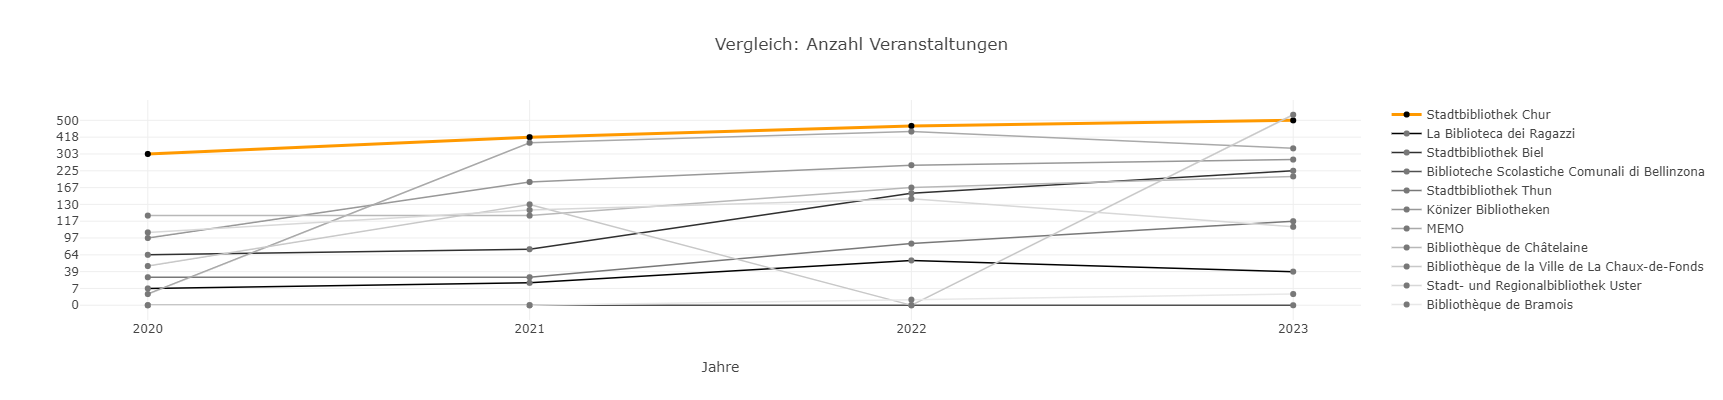
\includegraphics[angle=90,width=0.3\textwidth]{img/Abbildung01.PNG}
\caption{Abbildung 1: Beispiel aus dem Dashboard. Als Liniendiagramm
dargestellt wird hier die Zahl der Veranstaltungen, welche in der
Stadtbibliothek Chur in den Jahren 2020 bis 2023 durchgeführt wurden
(dargestellt durch die orange Linie, im Vergleich mit den zehn
vergleichbaren Bibliotheken).}
\end{figure}

Das Dashboard ist frei zugänglich im Netz verfügbar
(\url{https://bibliocheck.fhgr.ch} gehostet bei der Fachhochschule
Graubünden) und seine Existenz ist im schweizerischen Bibliothekswesen
bekannt gemacht worden. (Schuldt \& Schulze 2024)

\subsection{2.2 Datenqualität}\label{datenqualituxe4t}

Die Aussagekraft der Daten im Dashboard und weiterer Analysen, die mit
diesen Daten durchgeführt werden, hängt selbstverständlich von der
Datenqualität der Bibliotheksstatistik ab. Diese Daten werden von den
Bibliotheken selber geliefert. Das BfS scheint formelle Kontrollen
durchzuführen, auch wenn diese nicht öffentlich dokumentiert
sind.\footnote{Das \emph{Bundesamt für Statistik} unternimmt in den
  letzten Jahren Anstrengungen, die von ihm zur Verfügung gestellten
  Daten sichtbarer zu machen und zu dokumentieren. Aber viel Wissen über
  diese Daten musste in den letzten Jahren direkt beim Bundesamt oder
  anderen Personen erfragt werden (beispielsweise bei einem Kollegen des
  Autors, der für das BfS Fragen der Nutzung von Kulturdaten untersuchte
  und deshalb genaueren Einblick hatte). Der Autor hatte deshalb
  mehrfach direkten -- immer hilfreichen, offenen und schnellen --
  Kontakt mit dem Bundesamt, der aber vor allem informell passierte und
  deshalb nicht dokumentiert ist. Die in diesem Artikel getroffenen
  Aussagen sind, bis das BfS mehr Dokumentationen veröffentlicht, mit
  Vorsicht zu geniessen.}

Dennoch ist bei einem genaueren Blick in die Daten sichtbar, dass deren
Qualität nicht perfekt ist.

\begin{itemize}
\item
  Eine ganze Anzahl von Werten scheint eher auf Schätzungen zu beruhen
  als auf genauen Zählungen. So finden sich Werte, die über Jahre immer
  in Potenzen von Zehnern oder Hunderten ausgedrückt werden. Oder aber,
  Werte, bei denen immer gewisse Veränderungen zu erwarten wären (also
  nicht die Arbeitsplätze oder der Etat, die tatsächlich über längere
  Zeit gleich bleiben können), sind bei einigen Bibliotheken über Jahre
  konstant.
\item
  Es scheint auch, als ob Bibliotheken sich nicht genau an die
  Definitionen für die Variablen (Bundesamt für Statistik 2024) halten.
  Auch dabei ist zu vermuten, dass dies nicht absichtlich geschieht,
  aber es führt zu Inkonsistenzen. Ein offensichtliches Beispiel ist,
  dass es in der Schweiz eine ganze Anzahl von Bibliotheken gibt, welche
  gleichzeitig die Aufgaben mehrerer Bibliothekstypen wahrnehmen. In der
  Statistik sollten diese Bibliotheken alle diese Bibliothekstypen
  angeben, aber sie tun es nicht immer. Schnell sichtbar wird dies bei
  den Kantonsbibliotheken, welche gleichzeitig die Stadtbibliotheken der
  jeweiligen Hauptorte sind. (Das sind die Kantonsbibliotheken in
  Basel-Landschaft, Thurgau, Uri, Glarus, Obwalden, Schaffhausen,
  Schwyz, Solothurn und Zug.) In der Statistik verzeichnen sie sich aber
  alle nur als Kantonsbibliotheken. Durch die automatische Bearbeitung
  der Daten sind diese Bibliotheken -- jeweils die grössten allgemein
  öffentlichen Bibliotheken in ihrem Kanton -- jetzt nicht im Dashboard
  enthalten. Dies gilt aber auch umgekehrt für andere Bibliotheken, die
  offenbar die Bezeichnung «öffentlich» missverstehen. Eine ganze Anzahl
  von Spezialbibliotheken, die sich wohl als «nicht wissenschaftlich»
  verstehen, bezeichnet sich als «öffentlich». (Diese werden bei der
  Bearbeitung automatisch aus dem Datensatz entfernt.\footnote{Automatisch
    heisst hier, dass jeweils geschaut wird, ob in einer Gemeinde mehr
    als eine allgemein öffentliche Bibliothek existiert und wenn, dann
    wird die mit den meisten Nutzer*innen beibehalten, während die
    anderen entfernt werden. Aber dies ist eine unzufriedenstellende
    Lösung, die mehrere Annahmen trifft, zum Beispiel dass es in jeder
    Gemeinde höchstens eine allgemein öffentliche Bibliothek gibt. Das
    gilt beispielsweise für Neuchâtel nicht, wo neben der
    \emph{Bibliothéque publique et universitaire} -- die trotz dieses
    Namens heute nicht mehr mit der Universität des Kantons verbunden
    ist -- die \emph{Bibliothéque Ludothèque Pestalozzi} existiert,
    welche für Kinder und Jugendliche gedacht ist. Lange Zeit
    existierten aber auch in zweisprachigen Gemeinden -- beispielsweise
    Biel/Bienne -- pro Sprache eine Bibliothek und es kann nicht
    ausgeschlossen werden, dass dies nicht heute noch teilweise der Fall
    ist. Heute gibt es zudem eine anhaltende Entwicklung dazu, dass
    Gemeinden fusionieren und es ist nicht klar, ob dies dann jeweils
    für die Bibliotheken der fusionierenden Gemeinden gilt oder ob diese
    nicht -- vielleicht auch nur eine Zeit lang, bis alle Fragen geklärt
    sind -- nebeneinander existieren. Besser wäre es also, wenn die
    Daten in der Bibliotheksstatistik zumindest die richtigen
    Bibliothekstypen abbilden würden und damit solche nachträglichen
    Bereinigungen nicht mehr nötig wären.})
\end{itemize}

Eine weitere Herausforderung ist -- wie bei allen Bibliotheksstatistiken
--, dass die Vielfältigkeit der Bibliotheken vor Ort sich nie ganz mit
der Statistik deckt. Leicht sichtbar ist dies wieder daran, dass viele
Bibliotheken Aufgaben verschiedener Einrichtungen übernehmen, ohne dass
klar ist, wie diese Aufgaben in die Statistik «eingerechnet» werden
könnten. Wie gesagt, bezeichnen sich die neun Kantonsbibliotheken, die
auch allgemein öffentliche Bibliotheken sind, bislang nur als
Kantonsbibliotheken. Aber falls sie sich in Zukunft beiden
Bibliothekstypen zuordnen, wird nicht klar sein, ob -- und wenn ja, wie
-- sie diese Funktionen in der Statistik aufteilen können. Könnten Sie
zum Beispiel die Besuche der Stadtbibliothek und der Kantonsbibliothek
trennen? Oder sollen sie den Bestandsetat nach Aufgaben aufteilen? Wenn
nicht, liefern sie dann nicht Werte, die mit denen anderer Bibliotheken,
welche nicht die Aufgabe haben, Literatur aus und über den Kanton zu
erwerben, unvergleichbar sind?\footnote{In der Schweiz muss diese
  Literatur von den meisten damit beauftragten Bibliotheken erworben
  oder von Verlagen erbeten werden. Pflichtexemplargesetze existieren
  nur in den französischsprachigen Kantonen.}

Das gleiche Problem stellt sich bei kombinierten Schul- und
Gemeindebibliotheken, welche sich in der Schweiz recht oft finden und
die -- im Gegensatz zu reinen Schulbibliotheken, die als «nicht
öffentlich zugänglich» gelten -- an der Bibliotheksstatistik teilnehmen.
Was genau ist deren «Schulbibliotheksfunktion», für die sie oft einen
Budgetbeitrag von der Schule erhalten? Bislang soll dieser Wert nicht
«herausgerechnet» werden, aber ob Bibliotheken dies nicht trotzdem
irgendwie tun, ist ebenso unklar, wie der Effekt dieses «Hineinnehmens»
der Werte in die Bibliotheksstatistik. Kann man diese kombinierten
Bibliotheken wirklich fair mit «unkombinierten» allgemein öffentlichen
Bibliotheken vergleichen? Neben der Schulbibliotheksfunktion stellt sich
diese Frage auch für Ludotheken. Das sind in der Schweiz Einrichtungen,
in denen Spielzeug für Kleinkinder verliehen wird. Ludotheken existieren
praktisch in allen schweizerischen Gemeinden, in denen sich auch
allgemein öffentliche Bibliotheken befinden. Oft sind das getrennte
Organisationen, aber manchmal sind Bibliothek und Ludothek auch
miteinander verbunden (beispielsweise in der Stadtbibliothek Chur, wo
der Ludotheksteil geschätzt\footnote{Geschätzt vom Autor, der in dieser
  Stadt lebt und deshalb die Stadtbibliothek aus persönlicher Anschauung
  kennt.} 20\,\% der Gesamtfläche der Bibliothek einnimmt, also nicht zu
vernachlässigen ist). Bislang zeigt sich dies überhaupt nicht in den
Daten der Bibliotheksstatistik, obgleich es wohl Einfluss auf das
Budget, die Nutzer*innenstruktur und die Raumnutzung hat. Mit Wissen
über die konkreten Bibliotheken und lokalen Situationen lassen sich
zahlreiche weitere solche Grenzfälle und Fragen benennen.

Ein weiteres Problem ist, dass in der Schweiz eine ganze Anzahl von
Gemeinden zusammen eine allgemein öffentliche Bibliothek betreiben, ohne
dass dies in den Daten der Bibliotheksstatistik irgendwie sichtbar wäre.
Manchmal lässt sich dies aus den Namen der Bibliotheken schliessen,
beispielsweise bei der \emph{Bibliothek Rorschach-Rorschacherberg}, die
für beide eigenständigen Gemeinden, die in ihrem Namen genannt werden,
zuständig ist. Oft funktioniert dies aber auch nicht, beispielsweise bei
den Bibliotheken von Gemeinden um die Stadt Bern herum, die von den
\emph{Kornhausbibliotheken Bern} (Stadt Bern) im Auftrag der Gemeinden
als Standorte geführt werden (Bremgarten, Ittigen, Münchenbuchsee,
Münsingen, Gümlingen, Ostermundigen -- mit Ludothek --, Hinterkappelen,
Urtenen-Schönbühl, Worb und Zollikofen), aber in der
Bibliotheksstatistik nur unter den \emph{Kornhausbibliotheken Bern}
geführt werden. Gerade weil sich eine Anzahl von bibliothekarischen
Kennziffern auf die Gesamtzahl der Einwohner*innen im Umfeld der
jeweiligen Bibliothek bezieht, führt dies zu Verzerrungen.\footnote{Die
  Beispiele Rorschach-Rorschacherberg und \emph{Kornhausbibliotheken
  Bern} sind noch einfach zu recherchieren. Aber schon die Frage, ob
  eventuell andere Gemeinden den \emph{Kornhausbibliotheken} einen
  Beitrag bezahlen, damit deren Bewohner*innen auch die
  \emph{Kornhausbibliotheken} nutzen können, ist nur durch weitere
  Recherchen zu klären. (In diesem Fall auf der Homepage der
  \emph{Kornhausbibliotheken} (ohne Jahr).) Solche Vereinbarungen
  zwischen Gemeinden sind nicht selten, wechseln aber mit der Zeit. Für
  einen umfassenden Vergleich der Ergebnisse von Bibliotheken wäre es
  also notwendig, dass entweder eine ständig aktualisierte Liste von
  Gemeinden geführt würde, die auf solche Weise «zusammenspannen»
  (beispielsweise von den kantonalen Fachstellen oder dem
  Bibliotheksverband) oder aber, dass die Bibliotheken dies jedes Jahr
  bei der Abgabe ihrer Daten für die Bibliotheksstatistik meldeten.}

Zusammengefasst sind die Daten der Bibliotheksstatistik in sich
schlüssig, enthalten keine \linebreak grundsätzlichen Fehler, aber sie bilden nicht
die gesamte Realität der Bibliotheken ab. Zudem sind sie an Stellen
ungenau.\footnote{Über die letzten Jahre ist aber auch sichtbar, dass
  die Qualität besser geworden ist. Wie erwähnt, arbeitete der Autor vor
  zwei Jahren in einer Studie schon einmal mit diesen Daten. (Schuldt
  2022) Die Verbesserung der Qualität seitdem ist auffällig.
  Beispielsweise liefern die Bibliotheken immer mehr Werte, die mit den
  Definitionen übereinzustimmen scheinen. Kantonale Fachbeauftragte, der
  Bibliotheksverband \emph{bibliosuisse} und das BfS arbeiten, neben den
  Bibliotheken selber, daran, diese Daten zu verbessern.} Alle
Darstellungen, Vergleiche und Auswertungen müssen dies beachten: Die
Daten sind Annäherungen an die Realität, die allgemeine Trends zeigen.
Allerdings handelt es sich jetzt auch um Daten aus 622 unterschiedlichen
Bibliotheken. Diese Zahl erlaubt zu vermuten, dass einzelne Fehler oder
Ausnahmen keinen zu gross verzerrenden Einfluss haben.

\subsection{2.3 Sichtbare Trends}\label{sichtbare-trends}

Das Dashboard «BiblioCheck» ist frei zugänglich. Rückmeldungen aus
Bibliotheken zeigen \linebreak auch, dass daran ein Interesse besteht. Was genau
die Bibliotheken mit den Daten über sich selber tun, ist aber nicht
klar.

In diesem Abschnitt besprochen werden nicht diese Werte für einzelne
Bibliotheken, sondern nur die übergreifenden Trends, welche sich durch
die Zusammenfassung der Daten für die ganze Schweiz und über die vier
Jahre von 2020 bis 2023 zeigen. Sicherlich: Die Jahre 2020 bis
mindestens 2021 waren Jahre, die grösstenteils durch die COVID-19
Pandemie geprägt waren. Dies hatte wohl auch Einfluss auf die Nutzung
von Bibliotheken. Insoweit sind viele der Trends, die sich in den Daten
zeigen, mit Vorsicht zu geniessen. Besser wäre es, Daten von mindestens
drei «normalen» Jahren zu haben. Diese werden aber erst -- solange nicht
weitere vergleichbare Ereignisse wie die genannte Pandemie auftreten --
Ende des Jahres 2025 vorliegen (wenn man davon ausgeht, dass 2022 ein
«normales» Jahr war). Dennoch sind aus den Daten einige Trends sichtbar.

Die Bibliotheken, oder zumindest fast alle in der Bibliotheksstatistik
betrachteten Variablen, entwickeln sich stetig, wenn auch langsam, in
eine «gute Richtung». Das heisst, solche Werte wie die Besuche, die
aktiven Nutzer*innen, die Öffnungszeiten pro Woche, der Bestand, die
Anzahl der Arbeitsplätze, die geleisteten Arbeitsstunden des Personals,
aber auch der gesamte Etat oder der Etat pro Einwohner*in steigen
kontinuierlich leicht an. Das allgemein öffentliche Bibliothekswesen in
der Schweiz scheint recht gut aufgestellt zu sein. Das schliesst
selbstverständlich gegenläufige Entwicklungen in Einzelfällen nicht aus.
Aber im Ganzen scheint das, was die Bibliotheken tun, in ihrem
jeweiligen lokalen Rahmen gut zu funktionieren.

Dieser Anstieg der Werte erfolgt nicht sprunghaft, sondern in einer
stetigen, langsamen Entwicklung, die für einzelne Variablen auch
teilweise leichte Rückschritte enthält, welche sich dann im folgenden
Jahr wieder ausgleichen. Ein Beispiel dafür sind die Ausleihen pro
Bibliothek, deren Median (das gewichtete Mittel pro Daten)\footnote{Median
  ist der Wert, bei dem sich 50\,\% der Werte über und 50\,\% darunter
  befinden. Der Median ist weniger von Extremwerte beeinflusst als der
  Durchschnitt (welcher immer berechnet wird als die Summe aller Werte
  durch die Anzahl der Werte).} sich wie folgt entwickelte:

\begin{table}[]\centering
\begin{tabular}{|l|l|}
\hline
\textbf{Jahr} & \textbf{Wert (Median Ausleihe)} \\ \hline
2020          & 18.775                          \\ \hline
2021          & 19.256                          \\ \hline
2022          & 18.440                          \\ \hline
2023          & 20.309                          \\ \hline
\end{tabular}
\caption{Tabelle 1: Median der Ausleihen pro Bibliothek}
\end{table}

Der einzige Wert, welcher dieser Entwicklung einigermassen
entgegensteht, ist der Umsatz der Medien, welcher angibt, wie oft ein
Medium pro Jahr entliehen wurde. 2020 war dieser 2.0, erhöhte sich dann
für 2021 und 2022 auf 2.2, um 2023 wieder auf 2.0 zu fallen -- oder der,
anders interpretiert, praktisch stagniert. Aber: Es gibt keine
Vergleichswerte dazu, was ein guter oder schlechter Umsatz wäre, sondern
immer nur geschätzte Angaben. Ein zu kleiner Umsatz soll zeigen, dass
eine Bibliothek viele Medien hält, die kaum von Interesse für ihre
Nutzer*innen sind -- was im Falle der allgemein öffentlichen
Bibliotheken als problematisch gilt, in anderen Bibliotheken mit
Sammlungen oder speziellen Beständen für sehr spezifische
Nutzer*innengruppen nicht unbedingt --, während ein zu grosser Umsatz
zeige, dass die Bibliothek zu wenige Medien hält, für die ein grosses
Interesse existiert. Das führe zum schnellen Abnutzen dieser Medien und
langen Wartezeiten für die interessierten Nutzer*innen. Die Richtlinien,
welche der schweizerische Bibliotheksverband \emph{bibliosuisse}
herausgibt -- allerdings ohne anzugeben, wie die dort enthaltenen Zahlen
zustande kommen -- gibt für den Umsatz, den Bibliotheken erreichen
sollten, einen Wert von 3.5 an. (Vergleiche bibliosuisse 2020: 27)
Diesen Wert erreichen oder überschreiten aber nur 85 der 622
Bibliotheken, die im Dashboard ausgewertet sind. Für den
Bibliotheksverband könnte dies als Motivation gelten, diese Kennzahl bei
der Fortschreibung der Richtlinien genauer zu diskutieren: Ist sie
unrealistisch, weil sie von den meisten Bibliotheken nicht erreicht
wird? Oder ist das Bestandsmanagement in den schweizerischen
Bibliotheken nicht effektiv genug?

Durch die Aufteilung der Daten in die drei räumlichen Typen städtischer
Raum, Agglomeration und ländlicher Raum ist im Dashboard sichtbar, dass
es zwar erkennbare Unterschiede zwischen diesen drei Gruppen gibt, aber
dass die grundlegenden Tendenzen für sie alle zutreffen. Es ist zum
Beispiel nicht so, dass es nur in städtischen Bibliotheken
Veranstaltungen gibt oder einen steigenden Etat nur in Bibliotheken im
ländlichen Raum. Vielmehr sind die Unterschiede zwischen den Daten gut
durch die unterschiedlichen Ressourcen in den verschieden grossen
Gemeinden zu erklären. Dass zum Beispiel die durchschnittlichen
Öffnungszeiten in städtischen Bibliotheken (Median 2023: 22 Stunden /
Woche) höher sind, als in der Agglomeration (13 Stunden / Woche) oder im
ländlichen Raum (7 Stunden / Woche) ist zu erwarten, da die Bibliotheken
tendenziell auch jeweils grösser und besser mit Ressourcen ausgestattet
sind, je grösser die Gemeinden selber sind. Gleichzeitig deuten die
Daten für alle Raumtypen darauf hin, dass die Öffnungszeiten langsam,
aber doch stetig erhöht werden. Was als bibliothekspolitisches Thema zu
diskutieren wäre, ist, ob die Unterschiede zwischen diesen Räumen
gewollt und tragbar sind -- oder ob sie vielleicht ausgeglichen werden
müssten. Die Daten für die Bibliotheken zeigen vor allem, dass sich in
ihnen auch die unterschiedlichen Ressourcen, welche Gemeinden in der
Schweiz zur Verfügung stehen, zeigen.

\begin{figure}
\centering
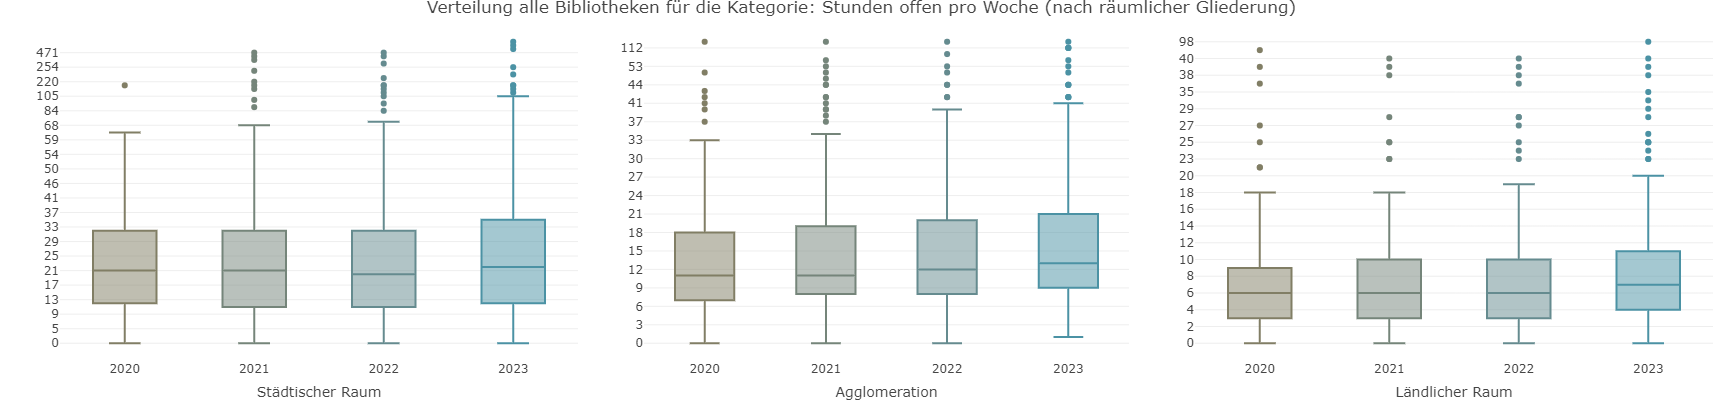
\includegraphics[angle=90,width=0.3\textwidth]{img/Abbildung02.PNG}
\caption{Abbildung 2: Beispiel aus dem Dashboard. Die Verteilung der
durchschnittlichen Öffnungszeiten pro Woche in den drei
unterschiedlichen Räumen. Zu beachten sind die unterschiedlichen Skalen
der drei Boxplots.}
\end{figure}

\section{3. Weitere Auswertungen}\label{weitere-auswertungen}

Die bislang dargestellten Ergebnisse sind direkt im Dashboard sichtbar.
Allerdings erlauben die Daten (immer mit den Einschränkungen, die in
Abschnitt 2.2 diskutiert wurden) weitere Auswertungen. Da es bislang
keine richtige Diskussion darüber gibt, welche Fragen mit Daten aus der
Bibliotheksstatistik beantwortet werden könnten, ist es auch nicht
wirklich möglich, hier an solche Diskussionen anzuschliessen.
Allerdings: Diese Fragen zu erarbeiten und zu begründen, würde eines
eigenen Beitrags bedürfen. Was in diesem Kapitel stattdessen getan
werden soll, ist, einige Möglichkeiten der Datenanalyse zu zeigen, die
recht einfach mithilfe von R umsetzbar sind.\footnote{Die Daten und das
  Skript sowie die vollständigen Auswertungen für alle vier Jahre sind
  frei zugänglich. (Schuldt 2024) In diesem Text werden aber nur einige
  Beispiele dargestellt.}

Die Darstellung der Daten in Liniendiagrammen, Boxplots und Tabellen,
wie sie im Dashboard angeboten werden, ist dabei selbstverständlich nur
eine Auswahl von Darstellungsmöglichkeiten. Daten lassen sich
bekanntlich auf sehr unterschiedliche Weise präsentieren. Die Frage ist
immer, was solche Darstellungen ermöglichen sollen.

Beispielsweise haben mehrere Kolleg*innen dem Autor vorgeschlagen, die
Daten im Dashboard auch auf einer Karte der Schweiz abzubilden. Das wäre
möglich, aber es wäre nicht klar, was damit erreicht würde. Die Karte
würde dann eigentlich nur zeigen, dass dort, wo viele Menschen wohnen,
auch viele Bibliotheken existieren. In dünnbesiedelten Gebieten, in der
Schweiz vor allem in den Bergregionen, würden sich weniger Bibliotheken
finden, die je mit weniger Ressourcen ausgestattet sind. Aber welche
Erkenntnisse sollten daraus gezogen werden? Sicherlich könnten die Daten
auf so einer Karte auch nach «Erfüllungsgraden» ausgewertet werden, wie
dies für Österreich in der \emph{Büchereilandkarte Österreich} vom
\emph{Büchereiverband Österreich} und dem \emph{Bundeskanzleramt} getan
wird. (bvoe 2023) Dort aber geschieht dies auf der Grundlage von
bibliothekspolitisch erarbeiteten Zielstandards, die in der Schweiz
nicht existieren.

\subsection{3.1 Verteilungen}\label{verteilungen}

Eine andere Darstellungsform, welche sich anbietet, ist die nach
Kantonen. Kantone sind in der Schweiz nicht nur politische Einheiten,
die teilweise Infrastrukturen für allgemein öffentliche Bibliotheken
unterhalten, sondern sie gelten gleichzeitig als identitätsstiftend für
die lokale Gesellschaft. Es wäre also interessant zu schauen, ob sich
bei einer Darstellung der Daten auf Kantonsebene Unterschiede zeigen,
die sich nicht auf andere Weise erklären lassen (also vor allem nicht
aus der Anzahl und Grösse der Gemeinden im jeweiligen Kanton).

In Abbildung 3 und 4 ist dies unternommen worden, einmal für den Etat
pro Einwohner*in im Jahr 2023 (Daten, die von 0 bis 180 CHF gestreut
sind) und einmal für die Besuche von Veranstaltungen im gleichen Jahr
(Daten, die von 0 bis 61.235 streuen).\footnote{Für die Kantone wurden
  die in der ISO 3166-2:CH definierten Abkürzungen verwendet, aber ohne
  die Länderkennzeichnung CH. Dies ist das Vorgehen, welches zum
  Beispiel auch das BfS nutzt. Die Anordnung der Kürzel (umgekehrt
  alphabetisch) wird von R vorgenommen und ist nicht einfach zu ändern.}

\begin{figure}
\centering
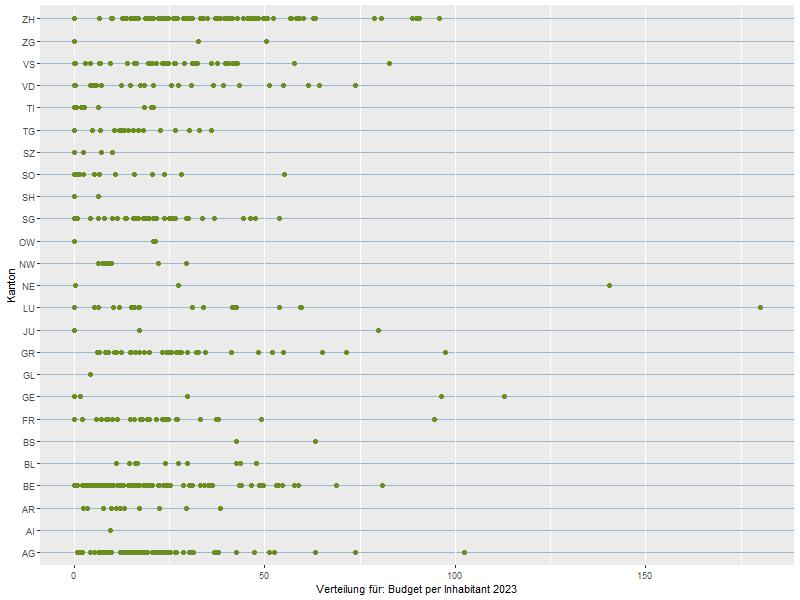
\includegraphics[angle=90,width=0.9\textwidth]{img/Abbildung03.JPG}
\caption{Abbildung 3: Verteilung der Daten für den Etat pro
Einwohner*in, 2023, nach Kantonen. Die einzelnen Punkte stellen jeweils
eine Wert -- also eine Bibliothek -- dar.}
\end{figure}

\begin{figure}
\centering
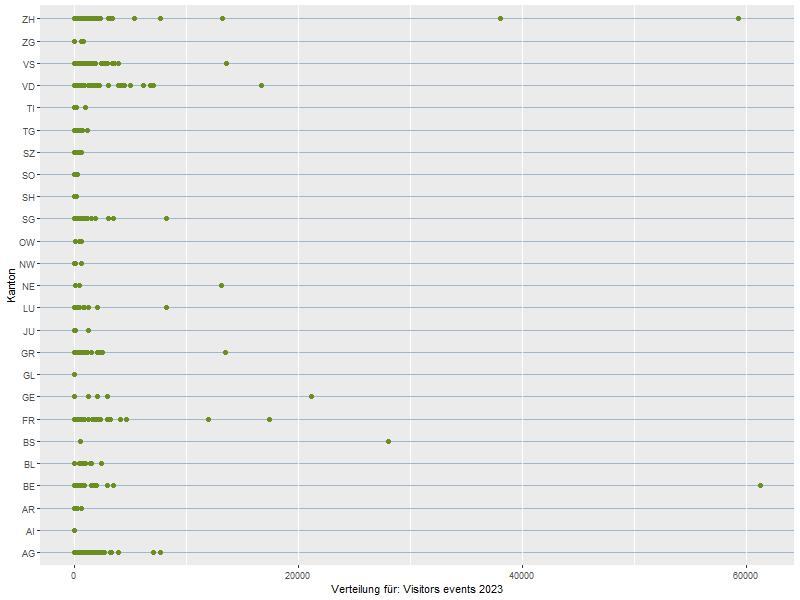
\includegraphics[angle=90,width=0.9\textwidth]{img/Abbildung04.JPG}
\caption{Abbildung 4: Verteilung der Daten für die Besuche von
Veranstaltungen, 2023, nach Kantonen. Die einzelnen Punkte stellen
jeweils eine Wert -- also eine Bibliothek -- dar.}
\end{figure}

Was lässt sich nun aus so einer Darstellung lesen? Zuerst wohl, dass
sich die Struktur der Schweiz in einige grosse und viele kleine
Gemeinden auch in den Daten zeigt. Dies ist in Abbildung 4 noch besser
zu sehen als in Abbildung 3. Hier zeigen nach rechts verschobene Punkte
immer grosse Gemeinden an (im Kanton Zürich beispielsweise Zürich und
Winterthur, im Kanton Bern die Stadt Bern). Grundsätzlich zeigen sich in
allen Kantonen, die eine herausragend grosse Gemeinde haben (unter
anderem Chur im Kanton Graubünden), diese Gemeinden in der Abbildung
auch mit eindeutig mehr Besuchen von Veranstaltungen. Der Grossteil der
Bibliotheken findet sich in dieser Darstellung aber links «am Rand»,
also mit einer vergleichbaren Zahl von Besuchen. Wenn diese
Darstellungen eines sichtbar machen, dann, dass die meisten Bibliotheken
in der Schweiz eher klein sind, dafür aber auch einigermassen
vergleichbare Ergebnisse haben.

Abbildung 3 zeigt aber auch, dass sich der Etat pro Einwohner*in viel
weiter «streut», als die Arbeitsergebnisse der Bibliotheken, für die
hier Abbildung 4 steht.\footnote{Dies zeigt sich auch für andere, hier
  nicht gesondert abgebildete Werte, wie Ausleihen oder aktive
  Nutzer*innen.} Zudem zeigten sich auch einige ohne Kontextwissen
unerklärliche Werte. Der Punkt ganz rechts ist zum Beispiel der Wert der
Bibliothek Vitznau im Kanton Luzern. Der Kanton ist eher als «sparsam»
bekannt (im Gegensatz zu den französischsprachigen Kantonen und den
«Stadtkantonen», die von einer Grossstadt dominiert werden). Es wäre
erstaunlich, wenn gerade diese Gemeinde überdurchschnittlich viel Geld
für ihre Bibliothek zahlt. Wenn es sich nicht um einen Fehler bei der
Eingabe der Daten handelt, ist eher zu vermuten, dass die Bibliothek
Geld von weiteren Gemeinden erhält, damit deren Bewohner*innen auch die
Bibliothek nutzen können. Sieht man aber von diesen Extremwerten ab,
zeigt die Darstellung vor allem, dass den Bibliotheken zwar
unterschiedlich viel Etat pro Einwohner*in zur Verfügung steht, aber
dass diese Unterschiede auch nicht sehr gross sind.

Solche Darstellungen lassen sich selbstverständlich auch für andere
Gruppen erstellen. Für die drei Raumtypen städtisch, Agglomeration und
ländlich ist dies einmal für die gleichen zwei Variablen wie eben
vorgenommen worden.

\begin{figure}
\centering
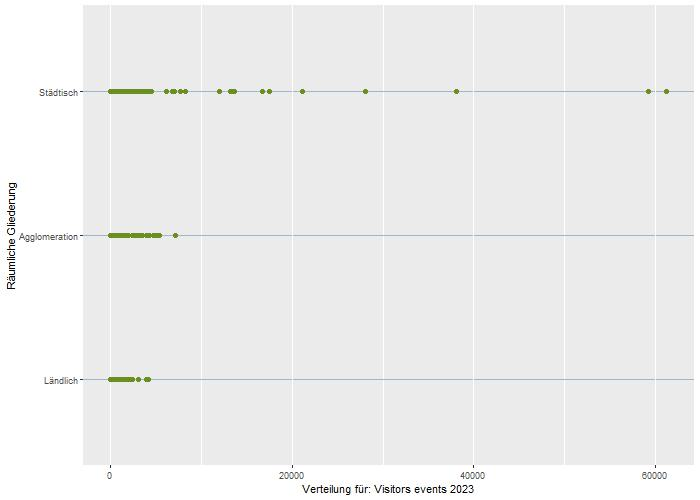
\includegraphics[angle=90,width=0.8\textwidth]{img/Abbildung05.JPG}
\caption{Abbildung 5: Verteilung der Daten für den Etat pro
Einwohner*in, 2023, nach Raumtypen. Die einzelnen Punkte stellen jeweils
eine Wert -- also eine Bibliothek -- dar.}
\end{figure}

\begin{figure}
\centering
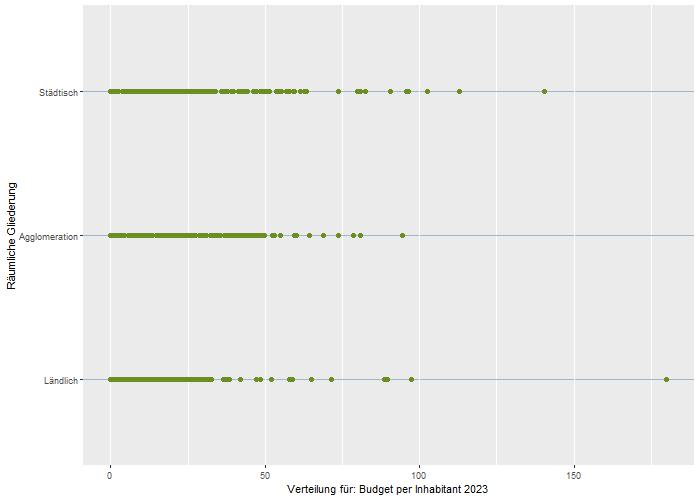
\includegraphics[angle=90,width=0.8\textwidth]{img/Abbildung06.JPG}
\caption{Abbildung 6: Verteilung der Daten für die Besuche von
Veranstaltungen, 2023, nach Raumtypen. Die einzelnen Punkte stellen
jeweils eine Wert -- also eine Bibliothek -- dar.}
\end{figure}

Auch dies zeigt Ergebnisse, die nach den bisherigen Darstellungen zu
erwarten sind: Bibliotheken in Städten haben tendenziell mehr Besuche
von Veranstaltungen als solche in der Agglomeration und auf dem Land.
Gleichzeitig stechen immer einige Bibliotheken als besonders aktiv
heraus, während der Grossteil der Bibliotheken eher ähnliche Ergebnisse
hat. Der Etat pro Einwohner*in hingegen verteilt sich einheitlicher über
die drei Raumtypen.

\subsection{3.2 Beschreibende Statistik}\label{beschreibende-statistik}

Eine weitere Form, Daten darzustellen, ist die beschreibende Statistik.
Damit erarbeitet man noch kein statistisches Modell, mit welchem
versucht werden könnte, den Einfluss von Variablen aufeinander zu
bestimmen. Dafür wären wieder weitere Vorarbeiten notwendig. Was
hingegen mit beschreibender Statistik möglich ist, ist zu bestimmen, ob
es einen direkt zu beobachtenden Unterschied zwischen verschiedenen
Gruppen (hier von Bibliotheken) gibt.

Um zu verdeutlichen, was damit untersucht werden könnte, sollen wieder
zwei Beispiele geliefert werden.\footnote{Genutzt wurde dafür die
  R-Bibliothek «compareGroups 4.0», welche den einfachen Vergleich von
  Gruppen ermöglicht.} In der folgenden Tabelle sind, wieder für 2023,
die Unterschiede zwischen den Bibliotheken in den drei Raumtypen
dargestellt.

Zu lesen ist die Tabelle wie folgt: In der ersten Spalte sind die
jeweiligen Variablen genannt, in der zweiten Spalte Werte für alle
Bibliotheken, gefolgt von drei Spalten mit den Werten für die
Bibliotheken in den drei Raumtypen. Die letzte Spalte gibt einen p-Wert
für die Entwicklungstendenz über die drei Raumtypen wieder. Die Werte in
der zweiten Zeile geben jeweils die Anzahl der Bibliotheken an. Zu sehen
ist zum Beispiel, dass die meisten Bibliotheken in Städten zu finden
sind (226) und die wenigsten im ländlichen Raum (182). Die Werte in den
restlichen Zeilen für alle Bibliotheken und die Raumtypen geben jeweils
den Median für die jeweilige Variable, auf die sich die Zeile bezieht,
an und dann in eckigen Klammern die Spannweite zwischen dem zweiten und
dritten Quartil. Das bedeutet, dass sich die Werte der 50\,\%
«durchschnittlichen» Bibliotheken zwischen den Werten in den Klammern
befinden, während die 25\,\% niedrigsten und höchsten Werte darunter
oder darüber liegen. Wird eine 0 angegeben -- beispielsweise bei «Number
visits 2023» -- heisst dies, dass ein Grossteil der Bibliotheken (über
25\,\%) einen Wert von 0 eingegeben haben (was in diesem Fall
unglaubwürdig ist und wohl eher zeigt, dass bislang viele Bibliotheken
ihre Besucher*innen nicht zählen).

Am interessantesten ist der p-Wert in der letzten Spalte. p-Werte geben
immer eine Signifikanz zur Nullhypothese an (die in diesem Fall lautet,
dass zwischen den drei miteinander verglichenen Gruppen keine
Unterschiede bestehen). Je kleiner dieser Wert ist, desto eher stimmt
diese Nullhypothese nicht. Oder, in unserem Fall: Je kleiner der p-Wert,
umso eher zeigt sich in den Daten, dass der Raumtyp einen Einfluss auf
die Werte der Bibliotheken hat. Allerdings: Was ein signifikanter Wert
ist -- also ab wann man davon ausgeht, dass ein gut begründeter
Zusammenhang besteht -- unterscheidet sich von Disziplin zu Disziplin
und von Fragestellung zu Fragestellung. Die p-Werte in dieser Tabelle
erscheinen fast durchgängig klein zu sein, also anders gesagt darauf
hinzuweisen, dass der Raumtyp einen massiven Einfluss darauf hat, wie
die Bibliotheken ausgestattet sind und welche Ergebnisse sie erreichen.
Aber: Heisst das tatsächlich, dass der Einfluss des Raumtyps auf die
Bibliotheken begründet -- also in gewisser Weise als «bewiesen» --
angesehen werden kann? (Immerhin zeigen sich ähnliche p-Werte auch für
die drei anderen Jahre, für die Daten vorliegen.) Ist die Datensammlung
aus 622 Bibliotheken überhaupt gross genug für eine solche Aussage? Und
selbst wenn ja, heisst das einfach, dass Bibliotheken im ländlichen Raum
der Schweiz einfach strukturell immer «abgehängt» sein werden? Ohne
weitere Vergleiche und klare Zielbestimmungen ist es nicht wirklich
möglich, dazu Aussagen zu treffen.\footnote{Auffällig ist auch der
  durchgehende Wert von «0» für das ehrenamtliche Personal. Hier zeigt
  sich wohl die Stärke des Medians im Vergleich zum Durchschnitt:
  Offenbar haben die meisten Bibliotheken (genauer: 475 von 622) gar
  kein ehrenamtliches Personal. Diejenigen mit ehrenamtlichem Personal
  finden sich alle im Bereich der obersten 25\,\%. Nur im ländlichen
  Raum gibt es eine grössere Anzahl mit (wenig) ehrenamtlichem Personal.
  Bei der Berechnung des Durchschnitts wären hier Werte erschienen, die
  schnell so interpretiert hätten werden können, als ob fast alle
  Bibliotheken ehrenamtliches Personal haben. Aber offenbar ist das
  meiste Personal in Bibliotheken in der Schweiz fest angestellt, wenn
  auch -- wie die Werte zu den Stellenprozenten zeigen -- oft mit einer
  geringen Stundenzahl.}

\begin{landscape}
\begin{table}[]\centering
\begin{tabular}{|l|l|l|l|l|l|}
\hline
                                 & \textbf{{[}ALL{]}}       & \textbf{Städtisch}        & \textbf{Agglomeration}   & \textbf{Ländlich}      & \textbf{p.overall} \\ \hline
                                 & N=622                    & N=226                     & N=214                    & N=182                  &                    \\ \hline
Number visits 2023               & \makecell{ 3610 \\ {[}0.00;16607{]}}    & \makecell{ 13242 \\ {[}0.00;32892{]}}    & \makecell{ 3912 \\ {[}0.00;13004{]}}    & \makecell{ 1378 \\ {[}0.00;3698{]}}   & \textless{}0.001   \\ \hline
Users 2023                       & \makecell{ 758 \\ {[}339;1451{]}}       & \makecell{ 1438 \\ {[}760;2678{]}}       & \makecell{ 772 \\ {[}414;1323{]}}       & \makecell{ 332 \\ {[}154;566{]}}      & \textless{}0.001   \\ \hline
Permanent staff 2023             & \makecell{ 4.00 \\ {[}3.00;5.00{]}}     & \makecell{ 5.00 \\ {[}3.00;7.00{]}}      & \makecell{ 4.00 \\ {[}3.00;5.00{]}}     & \makecell{ 3.00 \\ {[}2.00;4.00{]}}   & \textless{}0.001   \\ \hline
Permanent staff percentages 2023 & \makecell{ 0.80 \\ {[}0.30;1.60{]}}     & \makecell{ 1.65 \\ {[}0.86;2.70{]}}      & \makecell{ 0.85 \\ {[}0.40;1.30{]}}     & \makecell{ 0.30 \\ {[}0.10;0.60{]}}   & \textless{}0.001   \\ \hline
Volunteer staff 2023             & \makecell{ 0.00 \\ {[}0.00;0.00{]}}     & \makecell{ 0.00 \\ {[}0.00;1.00{]}}      & \makecell{ 0.00 \\ {[}0.00;0.00{]}}     & \makecell{ 0.00 \\ {[}0.00;1.00{]}}   & 0.02               \\ \hline
Opening hours per week 2023      & \makecell{ 13.0 \\ {[}8.00;25.0{]}}     & \makecell{ 22.0 \\ {[}12.2;35.0{]}}      & \makecell{ 13.0 \\ {[}9.00;21.0{]}}     & \makecell{ 7.00 \\ {[}4.00;10.8{]}}   & \textless{}0.001   \\ \hline
Budget 2023                      & \makecell{ 68734 \\ {[}17858;193870{]}} & \makecell{ 191770 \\ {[}58102;437138{]}} & \makecell{ 78022 \\ {[}22599;172581{]}} & \makecell{ 26128 \\ {[}6235;51812{]}} & \textless{}0.001   \\ \hline
Media budget 2023                & \makecell{ 14401 \\ {[}7000;28072{]}}   & \makecell{ 31056 \\ {[}15336;54960{]}}   & \makecell{ 15000 \\ {[}8767;23817{]}}   & \makecell{ 7012 \\ {[}3042;11550{]}}  & \textless{}0.001   \\ \hline
Collection physical 2023         & \makecell{ 10285 \\ {[}6616;16634{]}}   & \makecell{ 16696 \\ {[}11762;26640{]}}   & \makecell{ 10273 \\ {[}7698;14049{]}}   & \makecell{ 6208 \\ {[}4205;8609{]}}   & \textless{}0.001   \\ \hline
Collection digital 2023          & \makecell{ 14252 \\ {[}0.00;34918{]}}   & \makecell{ 17270 \\ {[}9305;34918{]}}    & \makecell{ 17270 \\ {[}0.00;34918{]}}   & \makecell{ 0.00 \\ {[}0.00;24784{]}}  & \textless{}0.001   \\ \hline
\end{tabular}
\caption{Tabelle 2, Teil 1: Vergleich der Variablen von Bibliotheken in den drei Raumtypen}
\end{table}
\end{landscape}

\begin{landscape}
\begin{table}[]\centering
\begin{tabular}{|l|l|l|l|l|l|}
\hline
                                 & \textbf{{[}ALL{]}}       & \textbf{Städtisch}        & \textbf{Agglomeration}   & \textbf{Ländlich}      & \textbf{p.overall} \\ \hline
                                 & N=622                    & N=226                     & N=214                    & N=182                  &                    \\ \hline
Seats 2023                       & \makecell{ 8.00 \\ {[}1.00;20.0{]}}     & \makecell{ 14.5 \\ {[}5.00;28.0{]}}      & \makecell{ 9.00 \\ {[}1.00;17.0{]}}     & \makecell{ 2.50 \\ {[}1.00;10.0{]}}   & \textless{}0.001   \\ \hline
Number events 2023               & \makecell{ 23.0 \\ {[}7.00;58.8{]}}     & \makecell{ 43.0 \\ {[}18.0;116{]}}       & \makecell{ 20.0 \\ {[}8.00;49.5{]}}     & \makecell{ 10.0 \\ {[}3.00;26.0{]}}   & \textless{}0.001   \\ \hline
Number of loans 2023             & \makecell{ 20362 \\ {[}8836;43386{]}}   & \makecell{ 44835 \\ {[}21094;76076{]}}   & \makecell{ 22483 \\ {[}13211;37602{]}}  & \makecell{ 7509 \\ {[}2694;14326{]}}  & \textless{}0.001   \\ \hline
Usage of ebooks 2023             & \makecell{ 144 \\ {[}0.00;3172{]}}      & \makecell{ 2724 \\ {[}0.00;6896{]}}      & \makecell{ 66.5 \\ {[}0.00;2610{]}}     & \makecell{ 0.00 \\ {[}0.00;354{]}}    & \textless{}0.001   \\ \hline
Visitors events 2023             & \makecell{ 259 \\ {[}0.00;828{]}}       & \makecell{ 575 \\ {[}7.00;1736{]}}       & \makecell{ 238 \\ {[}0.00;759{]}}       & \makecell{ 120 \\ {[}0.00;385{]}}     & \textless{}0.001   \\ \hline
Turnover 2023                    & \makecell{ 2.00 \\ {[}1.20;2.80{]}}     & \makecell{ 2.50 \\ {[}1.60;3.30{]}}      & \makecell{ 2.20 \\ {[}1.40;3.00{]}}     & \makecell{ 1.30 \\ {[}0.70;1.90{]}}   & \textless{}0.001   \\ \hline
Budget per Inhabitant 2023       & \makecell{ 18.4 \\ {[}6.90;29.8{]}}     & \makecell{ 20.8 \\ {[}9.30;33.8{]}}      & \makecell{ 19.2 \\ {[}7.10;31.1{]}}     & \makecell{ 14.7 \\ {[}5.70;24.1{]}}   & 0                  \\ \hline
Percent Active Users 2023        & \makecell{ 15.9 \\ {[}10.2;23.2{]}}     & \makecell{ 14.6 \\ {[}9.50;19.6{]}}      & \makecell{ 17.0 \\ {[}11.6;25.6{]}}     & \makecell{ 16.5 \\ {[}9.80;25.0{]}}   & 0                  \\ \hline
\end{tabular}
\caption{Tabelle 2, Teil 2: Vergleich der Variablen von Bibliotheken in den drei Raumtypen}
\end{table}
\end{landscape}

Trotzdem soll hier noch eine weitere Vergleichstabelle dargestellt
werden. In der Schweiz gibt es eine Anzahl von Kantonen, die eigene
Bibliotheksgesetze haben (Luzern, Schwyz, St.~Gallen), daneben eine
Anzahl von Kantonen, die zwar keine eigenen Bibliotheksgesetze haben,
aber Bibliotheken in anderen Gesetzen «mitregeln» oder aber Verordnungen
über Bibliotheken erlassen haben (Zürich, Bern, Graubünden, Aargau,
Thurgau, Jura). Die anderen Kantone haben keine solchen Regeln. Man
könnte vermuten, dass solche gesetzlichen Regelungen auch einen Einfluss
auf die Ressourcen haben, die Bibliotheken zur Verfügung gestellt werden
und damit auch auf die Ergebnisse der Bibliotheken. Solch eine Vermutung
lässt sich nun recht einfach anhand der vorliegenden Daten überprüfen,
wie in Tabelle 3 dargestellt. Die drei Gruppen, die hier überprüft
werden, sind die Kantone mit Bibliotheksgesetz («Yes»), mit anderen
gesetzlichen oder gesetzesähnlichen Regelungen über Bibliotheken
(«Bylaw») und die ohne solche Regelungen («No»).

Die Daten in Tabelle 3 zeigen jetzt aber diesen erwartbaren Zusammenhang
weniger, als den Zusammenhang zwischen den Raumtypen, wie er in Tabelle
2 dargestellt ist. Der p-Wert ist nur bei einigen Variablen in Tabelle 3
ähnlich klein, wie er es bei den meisten Variablen in Tabelle 2 ist.
Diese Variablen scheinen auch die zu sein, welche durch gesetzliche
Regelungen eher beeinflusst werden können: Budget, Personal oder der --
bei allgemein öffentlichen Bibliotheken in der Schweiz eh oft über die
Kantone oder Bibliotheksverbünde, nicht in den einzelnen Bibliotheken,
geregelte -- elektronische Bestand. Es scheint, dass mit gesetzlichen
Regelungen vor allem auf diese Variablen Einfluss genommen wird. Oder
aber, was auch eine mögliche Interpretation wäre, dass gesetzliche
Regelungen vor allem in Kantonen etabliert sind, die eher darauf achten,
dass die Bibliotheken einen ausreichenden Etat und Personal haben.
(Einzig der Zusammenhang zwischen den Regelungen und der Zahl der
Nutzer*innen, welcher sich auch in der Tabelle 3 zeigt, ist so nicht zu
erklären.)

Was solche Vergleiche ermöglichen, ist überhaupt einmal direkt nach
Zusammenhängen zu fragen. Zumeist werden diese im Bibliothekswesen eher
implizit und kaum dokumentiert gemacht (beispielsweise in Reden auf
Kongressen oder Gesprächen auf Apéros), also zum Beispiel beiläufig die
Vermutung geäussert, dass Bibliotheken in Städten besser ausgestattet
sind als auf dem Land oder dass Bibliotheksgesetze zu mehr Ressourcen
für Bibliotheken führen. Aber diese Vermutungen -- von denen es
zahlreiche weitere gibt -- sind kaum schriftlich dargelegt, begründet
oder gar empirisch abgesichert. Wenn aber Daten für solche Vergleiche
vorliegen, kann man nicht nur solche Vermutungen überprüfen, sondern
auch Annahmen über die sichtbaren Zusammenhänge anstellen, also zum
Beispiel zu klären versuchen, warum die gesetzlichen Regelungen einen
Einfluss auf die Zahl der Bibliotheksbesuche haben, aber offenbar keinen
auf die Zahl der Ausleihen oder die Besuche von
Veranstaltungen.\footnote{In diesem Text aus Platzgründen nicht
  dargestellt ist, dass sich in den vier Jahren, zu denen diese Daten
  jetzt vorliegen, zwar die einzelnen Werte, nicht aber die p-Werte
  geändert haben. Man kann also vermuten, dass sie das «normale
  Funktionieren» zeitgenössischer Bibliotheken in der Schweiz abbilden.}

\begin{landscape}
\begin{table}[]\centering
\begin{tabular}{|l|l|l|l|l|l|}
\hline
                                 & \textbf{{[}ALL{]}}       & \textbf{Yes}             & \textbf{Bylaw}           & \textbf{No}            & \textbf{p.overall} \\ \hline
                                 & N=622                    & N=77                     & N=341                    & N=204                  &                    \\ \hline
Number visits 2023               & \makecell{3610 \\ {[}0.00;16607{]}}    & \makecell{1045 \\ {[}0.00;17646{]}}    & \makecell{5106 \\ {[}520;17600{]}}     & \makecell{1790 \\ {[}0.00;11275{]}}  & \textless{}0.001   \\ \hline
Users 2023                       & \makecell{758 \\ {[}339;1451{]}}       & \makecell{1056 \\ {[}462;1835{]}}      & \makecell{759 \\ {[}371;1383{]}}       & \makecell{650 \\ {[}281;1448{]}}     & 0.02               \\ \hline
Permanent staff 2023             & \makecell{4.00 \\ {[}3.00;5.00{]}}     & \makecell{5.00 \\ {[}4.00;6.00{]}}     & \makecell{4.00 \\ {[}3.00;5.00{]}}     & \makecell{3.00 \\ {[}2.00;5.00{]}}   & \textless{}0.001   \\ \hline
Permanent staff percentages 2023 & \makecell{0.80 \\ {[}0.30;1.60{]}}     & \makecell{0.84 \\ {[}0.35;1.90{]}}     & \makecell{0.84 \\ {[}0.30;1.60{]}}     & \makecell{0.71 \\ {[}0.20;1.59{]}}   & 0.45               \\ \hline
Volunteer staff 2023             & \makecell{0.00 \\ {[}0.00;0.00{]}}     & \makecell{0.00 \\ {[}0.00;0.00{]}}     & \makecell{0.00 \\ {[}0.00;0.00{]}}     & \makecell{0.00 \\ {[}0.00;1.00{]}}   & 0.1                \\ \hline
Opening hours per week 2023      & \makecell{13.0 \\ {[}8.00;25.0{]}}     & \makecell{15.0 \\ {[}10.0;29.0{]}}     & \makecell{12.0 \\ {[}8.00;23.0{]}}     & \makecell{12.0 \\ {[}6.00;25.0{]}}   & 0.09               \\ \hline
Budget 2023                      & \makecell{68734 \\ {[}17858;193870{]}} & \makecell{84414 \\ {[}31700;253202{]}} & \makecell{84053 \\ {[}28300;211914{]}} & \makecell{34216 \\ {[}450;136186{]}} & \textless{}0.001   \\ \hline
Media budget 2023                & \makecell{14401 \\ {[}7000;28072{]}}   & \makecell{17081 \\ {[}10412;36000{]}}  & \makecell{15057 \\ {[}7651;30167{]}}   & \makecell{12546 \\ {[}4856;22928{]}} & 0                  \\ \hline
Collection physical 2023         & \makecell{10285 \\ {[}6616;16634{]}}   & \makecell{11457 \\ {[}7711;16904{]}}   & \makecell{9753 \\ {[}6395;14738{]}}    & \makecell{11998 \\ {[}6879;19960{]}} & 0.03               \\ \hline
Collection digital 2023          & \makecell{14252 \\ {[}0.00;34918{]}}   & \makecell{19503 \\ {[}0.00;34918{]}}   & \makecell{26545 \\ {[}11063;34918{]}}  & \makecell{0.00 \\ {[}0.00;9305{]}}   & \textless{}0.001   \\ \hline
\end{tabular}
\caption{Tabelle 3, Teil 1: Vergleich der Variablen von Bibliotheken in den drei Gesetzeslagen}
\end{table}
\end{landscape}

\begin{landscape}
\begin{table}[]\centering
\begin{tabular}{|l|l|l|l|l|l|}
\hline
                                 & \textbf{{[}ALL{]}}       & \textbf{Yes}             & \textbf{Bylaw}           & \textbf{No}            & \textbf{p.overall} \\ \hline
                                 & N=622                    & N=77                     & N=341                    & N=204                  &                    \\ \hline
Seats 2023                       & \makecell{8.00 \\ {[}1.00;20.0{]}}     & \makecell{3.00 \\ {[}1.00;19.0{]}}     & \makecell{8.00 \\ {[}2.00;20.0{]}}     & \makecell{10.0 \\ {[}1.00;20.0{]}}   & 0.13               \\ \hline
Number events 2023               & \makecell{23.0 \\ {[}7.00;58.8{]}}     & \makecell{17.0 \\ {[}6.00;41.0{]}}     & \makecell{21.0 \\ {[}8.00;50.0{]}}     & \makecell{28.0 \\ {[}6.00;86.5{]}}   & 0.11               \\ \hline
Number of loans 2023             & \makecell{20362 \\ {[}8836;43386{]}}   & \makecell{24663 \\ {[}13256;48991{]}}  & \makecell{21319 \\ {[}9206;43446{]}}   & \makecell{18621 \\ {[}6714;39745{]}} & 0.07               \\ \hline
Usage of ebooks 2023             & \makecell{144 \\ {[}0.00;3172{]}}      & \makecell{3323 \\ {[}849;5938{]}}      & \makecell{1132 \\ {[}0.00;3778{]}}     & \makecell{0.00 \\ {[}0.00;39.2{]}}   & \textless{}0.001   \\ \hline
Visitors events 2023             & \makecell{259 \\ {[}0.00;828{]}}       & \makecell{66.0 \\ {[}0.00;600{]}}      & \makecell{275 \\ {[}32.0;680{]}}       & \makecell{290 \\ {[}0.00;1399{]}}    & 0.01               \\ \hline
Turnover 2023                    & \makecell{2.00 \\ {[}1.20;2.80{]}}     & \makecell{2.50 \\ {[}1.58;3.12{]}}     & \makecell{2.20 \\ {[}1.30;2.90{]}}     & \makecell{1.60 \\ {[}1.00;2.40{]}}   & \textless{}0.001   \\ \hline
Budget per Inhabitant 2023       & \makecell{18.4 \\ {[}6.90;29.8{]}}     & \makecell{16.9 \\ {[}6.30;29.6{]}}     & \makecell{20.4 \\ {[}11.5;31.1{]}}     & \makecell{12.8 \\ {[}0.20;27.1{]}}   & \textless{}0.001   \\ \hline
Percent Active Users 2023        & \makecell{15.9 \\ {[}10.2;23.2{]}}     & \makecell{16.1 \\ {[}10.1;23.7{]}}     & \makecell{16.7 \\ {[}11.7;23.4{]}}     & \makecell{14.2 \\ {[}8.78;22.6{]}}   & 0.06               \\ \hline
\end{tabular}
\caption{Tabelle 3, Teil 2: Vergleich der Variablen von Bibliotheken in den drei Gesetzeslagen}
\end{table}
\end{landscape}


\subsection{3.3 Korrelationen}\label{korrelationen}

Noch eine Möglichkeit, Daten auszuwerten, ist, die einzelnen Variablen
miteinander in Korrelation zu setzen. Dabei geht es immer um die Frage,
wie stark der Zusammenhang zwischen zwei Variablen ist -- also in
unserem Fall zum Beispiel, ob die Zahl der Ausleihen wächst, wenn die
Zahl der Medien wächst oder ob die Höhe des Budgets sich auch bei der
Anzahl der Arbeitsplätze zeigt. Man kann sich dies in einem Diagramm
vorstellen, dessen x- und y-Achse jeweils eine der beiden miteinander
verglichenen Variablen abbildet. Im Diagramm wird nun ein Punkt für jede
Bibliothek eingetragen: Wenn auf der x-Achse das Budget und auf der
y-Achse die Zahl der Arbeitsplätze abgetragen ist, dann wird der Punkt
dort eingezeichnet, wo sich das Budget und die Zahl der Arbeitsplätze
treffen. Wenn alle Punkte (also Werte der Bibliotheken) im Diagramm
eingetragen sind, wird diejenige Linie durch das Diagramm gezogen,
welche am besten die Verteilung dieser Punkte einfängt: Wenn es einen
perfekten Zusammenhang gibt, also wenn in unserem Fall das Budget und
die Zahl der Arbeitsplätze in einem direkten Zusammenhang stehen, dann
müsste diese Linie perfekt in einem 90-Grad Winkel ansteigen. Wenn der
Zusammenhang perfekt, aber negativ ist -- also wenn zum Beispiel jeweils
weniger Budget zu jeweils mehr Besuchen in einer Bibliothek führte --,
dann müsste diese Linie genau anders herum gezogen sein. Bei anderen
Korrelationen ist diese Linie in einem anderen Winkel abzutragen.
Ausgedrückt werden Korrelationen durch Werte von 1 bis -1, wobei 1
heisst, dass die Korrelation perfekt positiv ist (also die Linie mit
einem Anstieg von 90 Grad abgetragen werden kann) und -1, dass die
Korrelation perfekt negativ ist. Je eher dieser Wert 0 ist, um so
geringer ist die Korrelation -- oder anders gesagt, um so weniger kann
man von einem Zusammenhang zwischen den beiden Werten ausgehen.

Selbstverständlich kann eine positive oder negative Korrelation noch
keine Erklärung sein -- manche können sich zufällig ergeben oder aber
durch einen anderen Zusammenhang erklärbar sein. Also beispielsweise
könnte sich ein positiver Zusammenhang zwischen der Anzahl des Personals
und der Anzahl der Medien in einer Bibliothek zeigen, der sich aber
dadurch erklären liesse, dass beide vom Budget der Bibliothek abhängen.
Aber erst, wenn wir die Korrelationen zwischen den Daten kennen, können
wir überhaupt darüber nachdenken, wie sich die Werte aufeinander
beziehen (und daraus zum Beispiel begründete bibliothekspolitische
Forderungen ableiten).

In Abbildung 7 ist nun eine Korrelationstabelle mit den Daten aus dem
Jahr 2023 dargestellt. Die Werte sind auch farblich gekennzeichnet -- je
höher sie sind (also je mehr 1), umso grüner sind sie. Negative
Korrelationen (also in Richtung -1) sind in Rot dargestellt. In der
Mitte jeder solcher Korrelationstabelle findet sich, wie auch in dieser,
eine durchgehende Linie von 1.0-Werten, die entsteht, weil hier die
Werte einer Variable mit sich selber in Korrelation gesetzt werden --
also zum Beispiel gefragt wird, ob die Zahl der Nutzer*innen im gleichen
Verhältnis steigt oder fällt, wie die Zahl der Nutzer*innen, was von
Natur aus immer eine perfekte Korrelation von 1.0 hervorbringt.

\begin{figure}
\centering
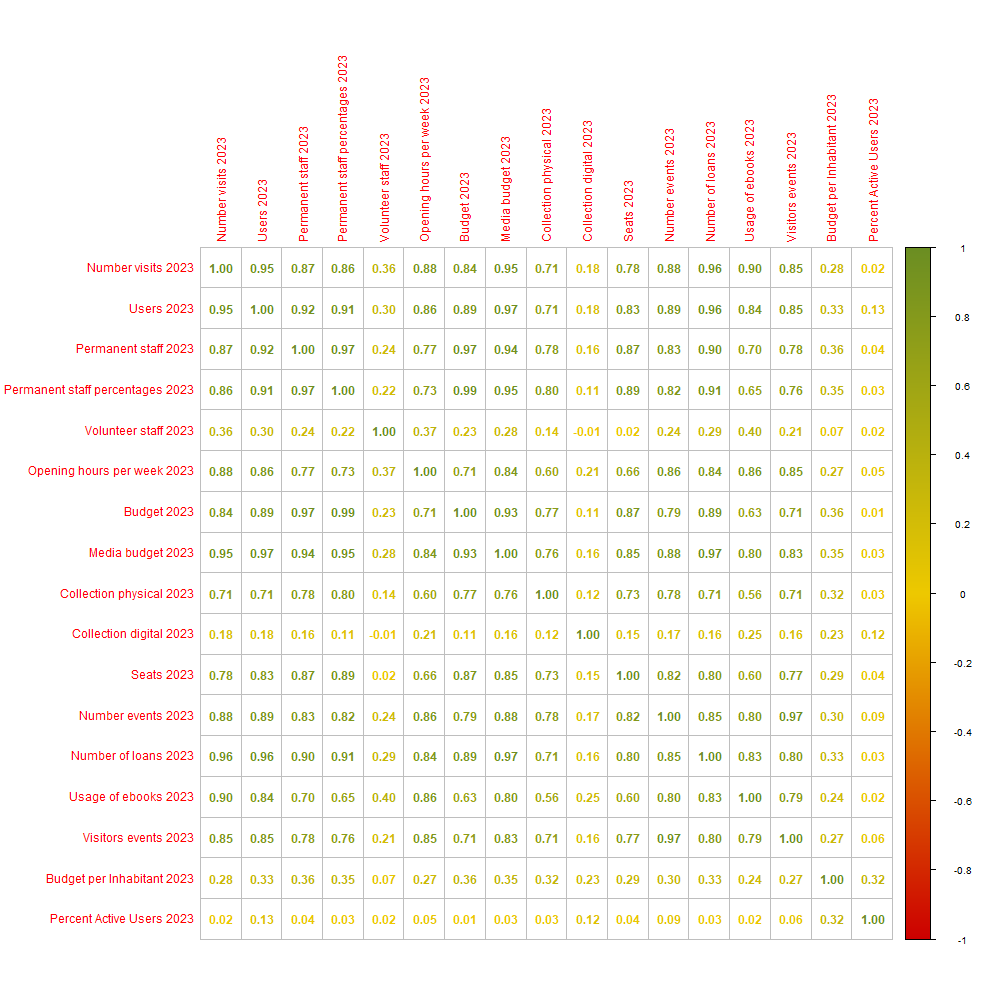
\includegraphics[width=0.99\textwidth]{img/Abbildung07.PNG}
\caption{Abbildung 7: Korrelationstabelle mit allen Variablen für die
Daten von 2023, numerische Darstellung.}
\end{figure}

Was in dieser Tabelle sofort auffällt, sind zwei Dinge: Erstens gibt es
keine negativen Korrelationen. Es gibt -- zumindest unter den
miteinander verglichenen Werten -- keine Situation, wo ein Wert fällt,
wenn ein anderer steigt. Zweitens fällt auf, dass der überwiegende Teil
der positiven Korrelationen recht hoch ist -- angezeigt durch Werte über
0.8 beziehungsweise durch ein dunkles Grün.

Man kann das (vorsichtig) so interpretieren, dass die Werte so eng
miteinander korrelieren, weil die Arbeit der Bibliotheken im Allgemeinen
gut auf die jeweiligen Ressourcen abgestimmt ist. Wenn zum Beispiel
grundsätzlich die Zahl der Ausleihen grösser ist, wenn auch das Budget
der Bibliothek grösser ist, heisst das wohl, dass alle Bibliotheken
insgesamt mit dem ihnen zur Verfügung stehenden Budget ungefähr so viele
Ausleihen erreichen, wie es in diesem Rahmen jeweils möglich ist. Oder
anders gesagt -- dass es nicht viele besser oder schlechter
funktionierende Bibliotheken gibt, sondern viele ähnlich gut
funktionierende, die sich vor allem durch ihre Ressourcen unterscheiden.

Interessant ist auch, welche Korrelationen offenbar weniger stark sind.
In Abbildung 8, in welcher die gleichen Werte noch einmal anders --
nämlich als Punkte, die grüner und grösser sind, je höher die
Korrelation ist (und die rot wären, wenn es negative Korrelationen gäbe)
-- dargestellt sind, werden diese «Ausnahmen» noch sichtbarer. Es ist
die Anzahl ehrenamtlichen Personals, die Zahl der elektronischen Medien,
der Etat pro Einwohner*in und der Anteil der Nutzer*innen an den
Einwohner*innen der jeweiligen Gemeinden. Diese haben offenbar einen
geringeren Einfluss auf die Ergebnisse der einzelnen Bibliotheken. Wie
ist dies zu erklären? Auch hier kann man nur vorsichtig interpretieren
und sollte tiefergehend forschen. Aber es scheint, dass die Bibliotheken
sehr gut für die Nutzer*innen funktionieren, die sie tatsächlich
erreichen -- also dass sie die vorhandenen Ressourcen (das Budget)
sinnvoll einsetzen für die Personen, welche die jeweilige Bibliothek
nutzen. Dabei ist es aber offenbar weniger wichtig, wie viele Personen
in der Gemeinde wohnen oder erreicht werden. Die schwache Korrelation
zwischen den digitalen Medien und den anderen Werten der Bibliotheken
scheint erklärbar dadurch, dass diese Medien eher auf Kantonsebene
lizenziert werden, also ihre Auswahl (die eh kaum möglich ist, da
grösstenteils die gleichen Lizenzen weniger Anbieter genutzt werden)
weniger an die Bibliotheken, deren Nutzer*innen und deren jeweiliges
lokales Umfeld angepasst sind als die physischen Medien. Die schwache
Korrelation mit dem ehrenamtlichen Personal lässt zumindest vermuten,
dass fest angestelltes (und dann auch oft bibliothekarisch aus- oder
zumindest weitergebildetes Personal) in den Bibliotheken eher zu
ähnlichen Arbeitsergebnissen führt, als wenn Arbeiten ehrenamtlich
übernommen werden. Man sollte das nicht so interpretieren, dass
ehrenamtliches Personal schlechter arbeiten würde, sondern wohl eher,
dass es bei seiner Arbeit eigene Schwerpunkte setzt (zum Beispiel mehr
auf Leseförderung als Veranstaltungsarbeit fokussiert) als fest
angestelltes Personal.\footnote{Gerade hier wäre eine Auswertung der
  deutschen und österreichischen Daten interessant, da dort
  ehrenamtliches Personal in den Bibliotheken teilweise einheitlichere
  Weiterbildungen erhält und gerade kirchlich getragene Bibliotheken oft
  auf mehr Infrastruktur zurückgreifen können als in der Schweiz.}

\begin{figure}
\centering
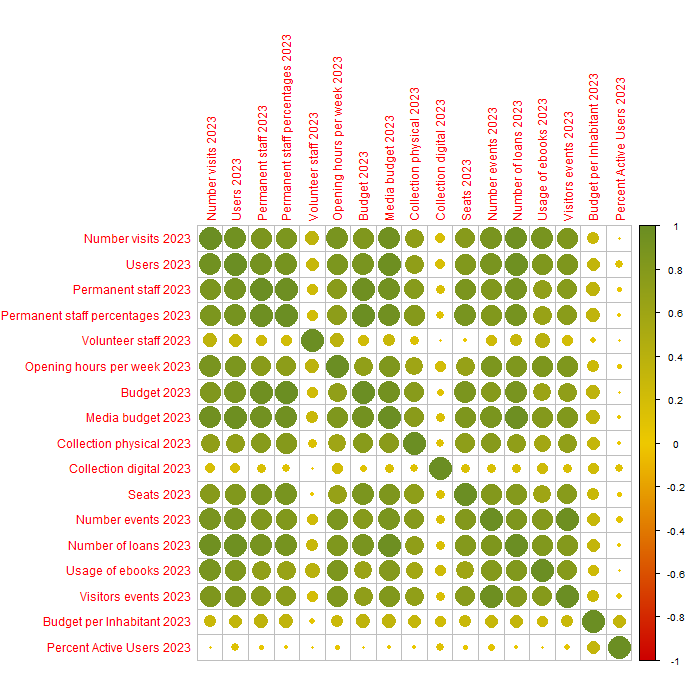
\includegraphics[width=0.99\textwidth]{img/Abbildung08.PNG}
\caption{Abbildung 8: Korrelationstabelle mit allen Variablen für die
Daten von 2023, graphische Darstellung.}
\end{figure}

\section{4. Fazit}\label{fazit}

In diesem Artikel wurde gezeigt, dass die Daten der schweizerischen
Bibliotheksstatistik -- hier beschränkt auf die der allgemein
öffentlichen Bibliotheken -- für mehr Fragen ausgewertet werden können,
als nur für den einfachen Vergleich ausgewählter Bibliotheken oder um
Argumente für bibliothekspolitische Forderungen zu liefern. Die Daten
sind jetzt vollständig genug und ausreichend gut, um für weitere
Forschung genutzt zu werden. Damit hat die schweizerische
Bibliotheksstatistik zu den nationalen Statistiken in Deutschland und
Österreich aufgeschlossen. Die Daten lassen sich mit recht einfachen
Mitteln auswerten. Der Autor dieses Textes -- welcher die gesamten hier
gezeigten Auswertungen vorgenommen hat -- hat keine besonderen
Kenntnisse in Statistik oder im Programmieren, konnte dies alles aber
mit einfachen Mitteln an einem durchschnittlich ausgestatteten Laptop
bewerkstelligen.

Sichtbar geworden ist aber, dass es an Diskussionen im Bibliothekswesen
darüber fehlt, was eigentlich die Annahmen über das Funktionieren von
Bibliotheken sind. Viele Fragen an die Daten lassen sich gar nicht
stellen, weil nicht klar ist, wie sich die Zusammenhänge zwischen, zum
Beispiel, der Zahl der Arbeitsplätze in Bibliotheken und der Nutzung der
Bibliothek zueinander verhalten. Zudem haben diese einfachen
Auswertungen wohl auch schon gezeigt, wie weit die bibliothekarischen
Diskussionen und die Daten in den Bibliotheksstatistiken auseinander
liegen. Mit der schweizerischen Bibliotheksstatistik lässt sich zum
Beispiel gar nicht untersuchen, ob die Grösse der Bibliotheken einen
Einfluss auf deren Nutzung hat, ganz abgesehen davon, ob und wenn ja wie
die Versuche von Bibliotheken, zu «Dritten Orten» zu werden, umgesetzt
werden und welchen Einfluss das auf die Arbeitsergebnisse der
Bibliotheken hat. Unsichtbar bleiben in den Daten zum Beispiel auch
Kinderaudiobooks wie \emph{TipTois}, \emph{Tonies} oder \emph{Lars, der
Lesebär}, welche in den letzten Jahren zu «Dauerrennern» in Bibliotheken
(und Buchhandlungen) geworden sind, aber bei denen nicht klar ist, wo in
den Daten überhaupt deren «Nutzung» eingetragen ist. Auch die
zahlreichen in den letzten Jahren eingerichteten «Bibliotheken der
Dinge» sind in den Daten nicht sichtbar.

Letztlich ist dieser Text ein Aufruf, gerade an statistisch versierte
Kolleg*innen, Forschende und Personen, die in der bibliothekarischen
Ausbildung Abschlussarbeiten schreiben, die Daten der
Bibliotheksstatistiken für mehr und diversere Fragen zu nutzen als
bisher. Sie haben das Potential, mehr darüber zu zeigen, wie
Bibliotheken funktionieren, welche sinnvollen bibliothekspolitischen
Forderungen gestellt werden können und auch, was von Bibliotheken an
Arbeitsergebnissen erwartet werden kann.

\section{Literatur}\label{literatur}

Bibliosuisse (2020). \emph{Richtlinien Öffentliche Bibliotheken.
Grundlagen und Empfehlungen zu Personal, Infrastruktur, Angeboten und
Leistungen. Qualitätsmanagement.} Aarau: Bibliosuisse, 2020,
\url{https://www.bibliosuisse.ch/DesktopModules/EasyDNNNews/DocumentDownload.ashx?portalid=0&moduleid=729&articleid=37&documentid=1}
Zugriff: 08.10.2024

Bundesamt für Statistik (2024). \emph{Definitionen der Variablen der
Schweizerischen Bibliotheksstatistik: Referenzdaten und Definitionen der
Variablen}. Neuchâchtel: Bundesamt für Statistik,
\url{https://dam-api.bfs.admin.ch/hub/api/dam/assets/30645434/master}
Zugriff: 08.10.2024

Bundesamt für Statistik (ohne Jahr, a). \emph{Räumliche Typologien},
\url{https://www.bfs.admin.ch/bfs/de/home/statistiken/querschnittsthemen/raeumliche-analysen/raeumliche-gliederungen/raeumliche-typologien.html}
Zugriff: 08.10.2024

Bundesamt für Statistik (ohne Jahr, b). \emph{Nutzungsbedingungen}.
\url{https://www.bfs.admin.ch/bfs/de/home/bfs/bundesamt-statistik/nutzungsbedingungen.html}
Zugriff: 08.10.2024

bvoe (2023). \emph{Büchereilandkarte}.
\url{https://www.bvoe.at/ndrp/buechereilandkarte/} Zugriff: 08.10.2024

dbv (ohne Jahr). \emph{Publikationen}.
\url{https://www.bibliotheksverband.de/publikationen} Zugriff:
08.10.2024

ISO (Hrsg.) (2022). \emph{ISO 2789:2022: Information and documentation
--- International library statistics}. Vernier: International
Organization for Standardization, 2022

Kornhausbibliotheken (ohne Jahr). \emph{Der Bibliotheksverbund}.
\url{https://www.kob.ch/die-kornhausbibliotheken/region-bern-mittelland/}
Zugriff: 08.10.2024

Schuldt, Karsten (2022). \emph{Waren Öffentliche Bibliotheken im
DACH-Raum 2020 in einer Krise?: Ein Blick auf die
Bibliotheksstatistiken}. In: Informationspraxis 8 (2022) 1,
\url{https://doi.org/10.11588/ip.2022.1.89240}

Schuldt, Karsten (2024). \emph{Data for the Article "Einige Anmerkungen
zur schweizerischen Bibliotheksstatistik"}.
\url{https://doi.org/10.5281/zenodo.13937880}

Schuldt, Karsten ; Schultze, Simon (2024). \emph{Ein Dashboard für die
ÖBs der Schweiz}. In: Bibliosusse info 6 (2024) 2: 21

Stieber, Martin (2024). \emph{Statistik öffentlicher Bibliotheken. Die
Zahlen aus der Zeit vor der Corona-Pandemie rücken in Reichweite.} In:
Büchereiperspektiven (2024) 1: 52--55

Stieber, Martin (2023). \emph{Statistik öffentlicher Bibliotheken. Mit
viel Einsatz aus der Pandemie}. In: Büchereiperspektiven (2023) 1:
52--55

%autor
\begin{center}\rule{0.5\linewidth}{0.5pt}\end{center}

\textbf{Dr. Karsten Schuldt}, ist Wissenschaftlicher Projektleiter am
Institut für Informationswissenschaft, FH Graubünden und Redakteur der
LIBREAS. Library Ideas.

\end{document}